\chapter{Tinjauan Pustaka}


\section{Embedded systems dan IoT}
The term IoT (Internet of Things) is recent but refers to an old usage called Machine-to-Machine.
Machine-to-Machine (M2M) is a set of wired or wireless network technologies that allow the
automatic exchange of information between systems without human intervention. The IoT is simply
a wider vision of M2M, where the devices don't only come from the industrial world, but also from
common public usage.
The IoT market continues to grow significantly around the world. This rapid evolution encourages
new players to propose new technologies at each stage: the development of hardware devices,
connectivity coverage, and cloud services (i.e., data storage of visualization platforms).
The IoT is often presented as the new industrial revolution, and marketing often promises that all
use cases are "smart": smart building, smart city, smart healthcare, etc. However, making things
“smart” is not always easy and many protocols exist.

\subsection{Embedded System}
Embedded systems are specialized computing systems that are designed to perform dedicated functions within a larger system. They are typically characterized by their integration into the devices they control, real-time operation, and resource constraints (e.g., limited processing power, memory, and energy consumption). Embedded systems can be found in a wide range of applications, from consumer electronics (e.g., smartphones, smart appliances) to industrial automation (e.g., robotics, process control).

In the context of IoT, embedded systems play a crucial role as the "things" that collect and process data from the environment. They often include sensors, actuators, and communication interfaces that enable them to interact with other devices and the cloud. The design and development of embedded systems for IoT applications require careful consideration of factors such as connectivity, interoperability, security, and power management.

Generally speaking, electronic systems can be characterized by their power consumption,
computing power, size, and price. In the specific case of embedded systems used in IoT, we can
assign the following weight to each of the characteristics:

While there are certainly exceptions to this simple definition, we assume that, compared to other
electronic systems, embedded systems used in IoT have:
\begin{enumerate}
    \item Low-power consumption
    \item Low computing power
    \item A small size
    \item A low price
\end{enumerate}
These characteristics are often interdependent. For example, a small size usually implies a low
power consumption and a low price. Similarly, a low power consumption often implies a low
computing power. The design of embedded systems is often a trade-off between these different
characteristics, depending on the specific application and requirements.

\subsection{The IoT wireless protocols}
The IoT wireless protocols can be classified into three main categories based on their range and data rate: short-range, medium-range, and long-range protocols.
\begin{itemize}
    \item Short-range protocols: These protocols are designed for communication over short distances, typically within a few meters. They are commonly used for personal area networks (PANs) and home automation applications. Examples of short-range protocols include Bluetooth, Zigbee, and Wi-Fi.
    \item Medium-range protocols: These protocols are designed for communication over moderate distances, typically up to a few hundred meters. They are commonly used for local area networks (LANs) and industrial automation applications. Examples of medium-range protocols include Wi-Fi, Z-Wave, and Thread.
    \item Long-range protocols: These protocols are designed for communication over long distances, typically several kilometers or more. They are commonly used for wide area networks (WANs) and smart city applications. Examples of long-range protocols include LoRaWAN, Sigfox, and NB-IoT.
\end{itemize}
Each of these protocols has its own advantages and disadvantages, and the choice of protocol depends on the specific requirements of the IoT application, such as range, data rate, power consumption, and cost

Sigfox and LoRaWAN are considered extremely long range and extremely low-power protocols. These types of networks are all referred to as Low Power
Wide Area Network (LPWANs). In this research, we focus on LoRaWAN (Long Range Wide Area Network) which is a long range
standard that uses a low data-rate with low power consumption needs.

\section{An Overview of LoRaWAN Fundamentals and Architecture}

LoRaWAN is a Low Power Wide Area Network (LPWAN) protocol designed to support long-range, low-power, and low-data-rate communication for Internet of Things (IoT) applications. Developed and maintained by the LoRa Alliance, the protocol defines the Media Access Control (MAC) layer that operates over the physical layer provided by LoRa modulation. Since its initial release in January 2015, LoRaWAN has evolved through multiple specification versions, with LoRaWAN 1.0.4 and 1.1 representing the latest stable iterations at the time of writing.

This section provides a concise technical overview of LoRaWAN fundamentals, including its key characteristics, architecture, communication model, security mechanisms, and typical application domains.

\subsection{Key Characteristics of LoRaWAN}
LoRaWAN exhibits several defining features that make it particularly well-suited for IoT deployments:
\begin{enumerate}
    \item \textbf{Long Range}: Communication ranges of up to 10+ km in rural environments and 2–5 km in dense urban settings are achievable, depending on terrain and interference conditions.
    \item \textbf{Low Power Consumption}: End devices can operate for 5–10 years or more on a single battery due to optimized duty cycling and sleep modes.
    \item \textbf{Secure Communication}: End-to-end data confidentiality and integrity are ensured through AES-based symmetric encryption.\item \textbf{Bidirectional Communication}: The protocol supports both uplink (device-to-server) and downlink (server-to-device) messaging.
    \item \textbf{Bidirectional Communication}: The protocol supports both uplink (device-to-server) and downlink (server-to-device) messaging.
    \item \textbf{Scalability}: LoRaWAN networks can support millions of devices per gateway due to its ALOHA-based access scheme and adaptive data rate (ADR) mechanisms.
    \item \textbf{Geolocation Support}: LoRaWAN enables device geolocation without GPS through time difference of arrival (TDOA) techniques using multiple gateways.
    \item \textbf{Adaptive Data Rate (ADR)}: The protocol dynamically adjusts data rates and transmission power based on link quality to optimize network capacity and battery life.
    \item \textbf{Global Standardization}: LoRaWAN is standardized by the LoRa Alliance, ensuring interoperability across devices and networks worldwide.
\end{enumerate}

\subsection{Data Rate and Payload Constraints}
LoRaWAN is optimized for small, infrequent data transmissions. Key constraints include:
\begin{enumerate}
    \item \textbf{Payload Size}: Ranges from 51 to 242 bytes per message, depending on regional regulations and the selected data rate.
    \item \textbf{Data Rate}: Varies between 0.3 kbps and 50 kbps, determined by the spreading factor (SF) and bandwidth configuration.
    \item \textbf{Message Frequency}: Devices are typically designed to transmit 1–100 messages per day.
    \item \textbf{Duty Cycle}: Subject to national regulatory limits (e.g., 1\% in Europe under ETSI regulations).
    \item The spreading factor is a critical transmission parameter that trades off data rate against communication range and robustness: higher spreading factors (e.g., SF12) enable longer-range communication at the expense of lower throughput, whereas lower spreading factors (e.g., SF7) support higher data rates over shorter distances.
\end{enumerate}

\subsection{Typical Application Domains}
LoRaWAN is widely adopted in scenarios that demand long battery life, extended coverage, cost efficiency, and minimal data exchange. Representative use cases include:

\begin{enumerate}
    \item \textbf{Smart Agriculture}: Soil moisture monitoring, crop health tracking, livestock management.
    \item \textbf{Environmental Monitoring}: Air quality sensing, water level monitoring, weather stations.
    \item \textbf{Smart Buildings}: HVAC control, lighting management, occupancy sensing.
    \item \textbf{Asset Tracking}: Fleet management, inventory tracking, cold chain monitoring.
    \item \textbf{Smart Cities}: Street lighting control, traffic and parking monitoring, waste management.
    \item \textbf{Agriculture}: Soil moisture sensing, irrigation automation, livestock tracking.
    \item \textbf{Supply Chain and Logistics}: Asset tracking, cold chain monitoring, inventory management.
    \item \textbf{Utilities}: Smart metering for water, gas, and electricity; leak and tamper detection.
    \item \textbf{Industrial IoT}: Condition monitoring, predictive maintenance, environmental sensing.
\end{enumerate}

\subsection{LoRa vs. LoRaWAN}
It is essential to distinguish between LoRa and LoRaWAN:
\begin{enumerate}
    \item \textbf{LoRa} is a proprietary physical layer modulation technique based on Chirp Spread Spectrum (CSS). It encodes data using linear frequency-modulated chirp pulses, offering high link budgets and resilience to multipath fading and Doppler shifts.
    \item \textbf{LoRaWAN} is a MAC-layer protocol that defines how LoRa-enabled devices access the network, structure messages, manage sessions, and ensure security. It standardizes device behavior across heterogeneous deployments and enables interoperability.
\end{enumerate}
Thus, LoRa provides the physical transmission mechanism, while LoRaWAN governs the network-level communication rules.

\subsection{Network Architecture}
A standard LoRaWAN network comprises four primary components:

\begin{enumerate}
    \item \textbf{End Devices}: Sensor or actuator nodes that generate or receive application data. They communicate wirelessly using LoRa modulation.
    \item \textbf{Gateways}: Multi-channel, multi-modem transceivers that receive uplink messages from end devices and forward them to the Network Server via backhaul (e.g., Ethernet, cellular). Gateways also relay downlink messages from the server to end devices.
    \item \textbf{Network Server (LNS)}: Centralized software responsible for network management, including message deduplication, adaptive data rate (ADR) control, and routing.
    \item \textbf{Application Server}: Processes decrypted application-layer data and interfaces with end-user services or dashboards.
\end{enumerate}

\subsection{Message Flow}
LoRaWAN employs a star-of-stars topology, where end devices communicate directly with multiple gateways. The message flow can be summarized as follows:
\subsubsection{Uplink Communication}
Uplink messages originate at end devices and are transmitted over the air using an ALOHA-based random access scheme—no pairing with specific gateways is required. All gateways within radio range receive the message and forward it to the Network Server. The server performs deduplication by retaining only one copy of redundant receptions and then separates network-layer and application-layer payloads.
\subsubsection{Downlink Communication}
Downlink messages are initiated by the Network or Application Server and scheduled for transmission during predefined receive windows (RX1 and RX2) following an uplink. The Network Server selects an appropriate gateway to deliver the message based on link quality and timing constraints.

\subsection{Security Model}
LoRaWAN employs a two-layer symmetric key encryption scheme to ensure separation of concerns between network and application functions:

\begin{enumerate}
    \item \textbf{Network Session Key (NwkSKey)}: Encrypts MAC commands and ensures integrity of network-layer payloads. Known only to the end device and Network Server.
    \item \textbf{Application Session Key (AppSKey)}: Encrypts application data. Shared exclusively between the end device and Application Server.
\end{enumerate}
These session keys are derived from root keys during the join procedure (either Over-the-Air Activation—OTAA—or pre-provisioned Activation-by-Personalization—ABP). Session keys are rotated upon re-joining the network, enhancing forward secrecy.

\subsection{The Things Stack}
The Things Stack is an enterprise-grade, open-source implementation of a LoRaWAN Network Server that integrates both Network Server and Application Server functionalities. It supports secure onboarding, management, and monitoring of millions of LoRaWAN devices at scale. By abstracting low-level protocol details, The Things Stack enables rapid deployment of production-grade LoRaWAN solutions across diverse verticals.
LoRaWAN represents a robust, standardized, and scalable solution for LPWAN-based IoT deployments. Its combination of long-range capability, energy efficiency, strong security, and regulatory adaptability has driven global adoption across smart infrastructure, agriculture, logistics, and industrial automation. Understanding its layered architecture—spanning physical modulation (LoRa), MAC protocol (LoRaWAN), and network software (e.g., The Things Stack)—is essential for designing and deploying reliable IoT systems.



\section{LoRaWAN Architecture}
\begin{figure}
    \centering
    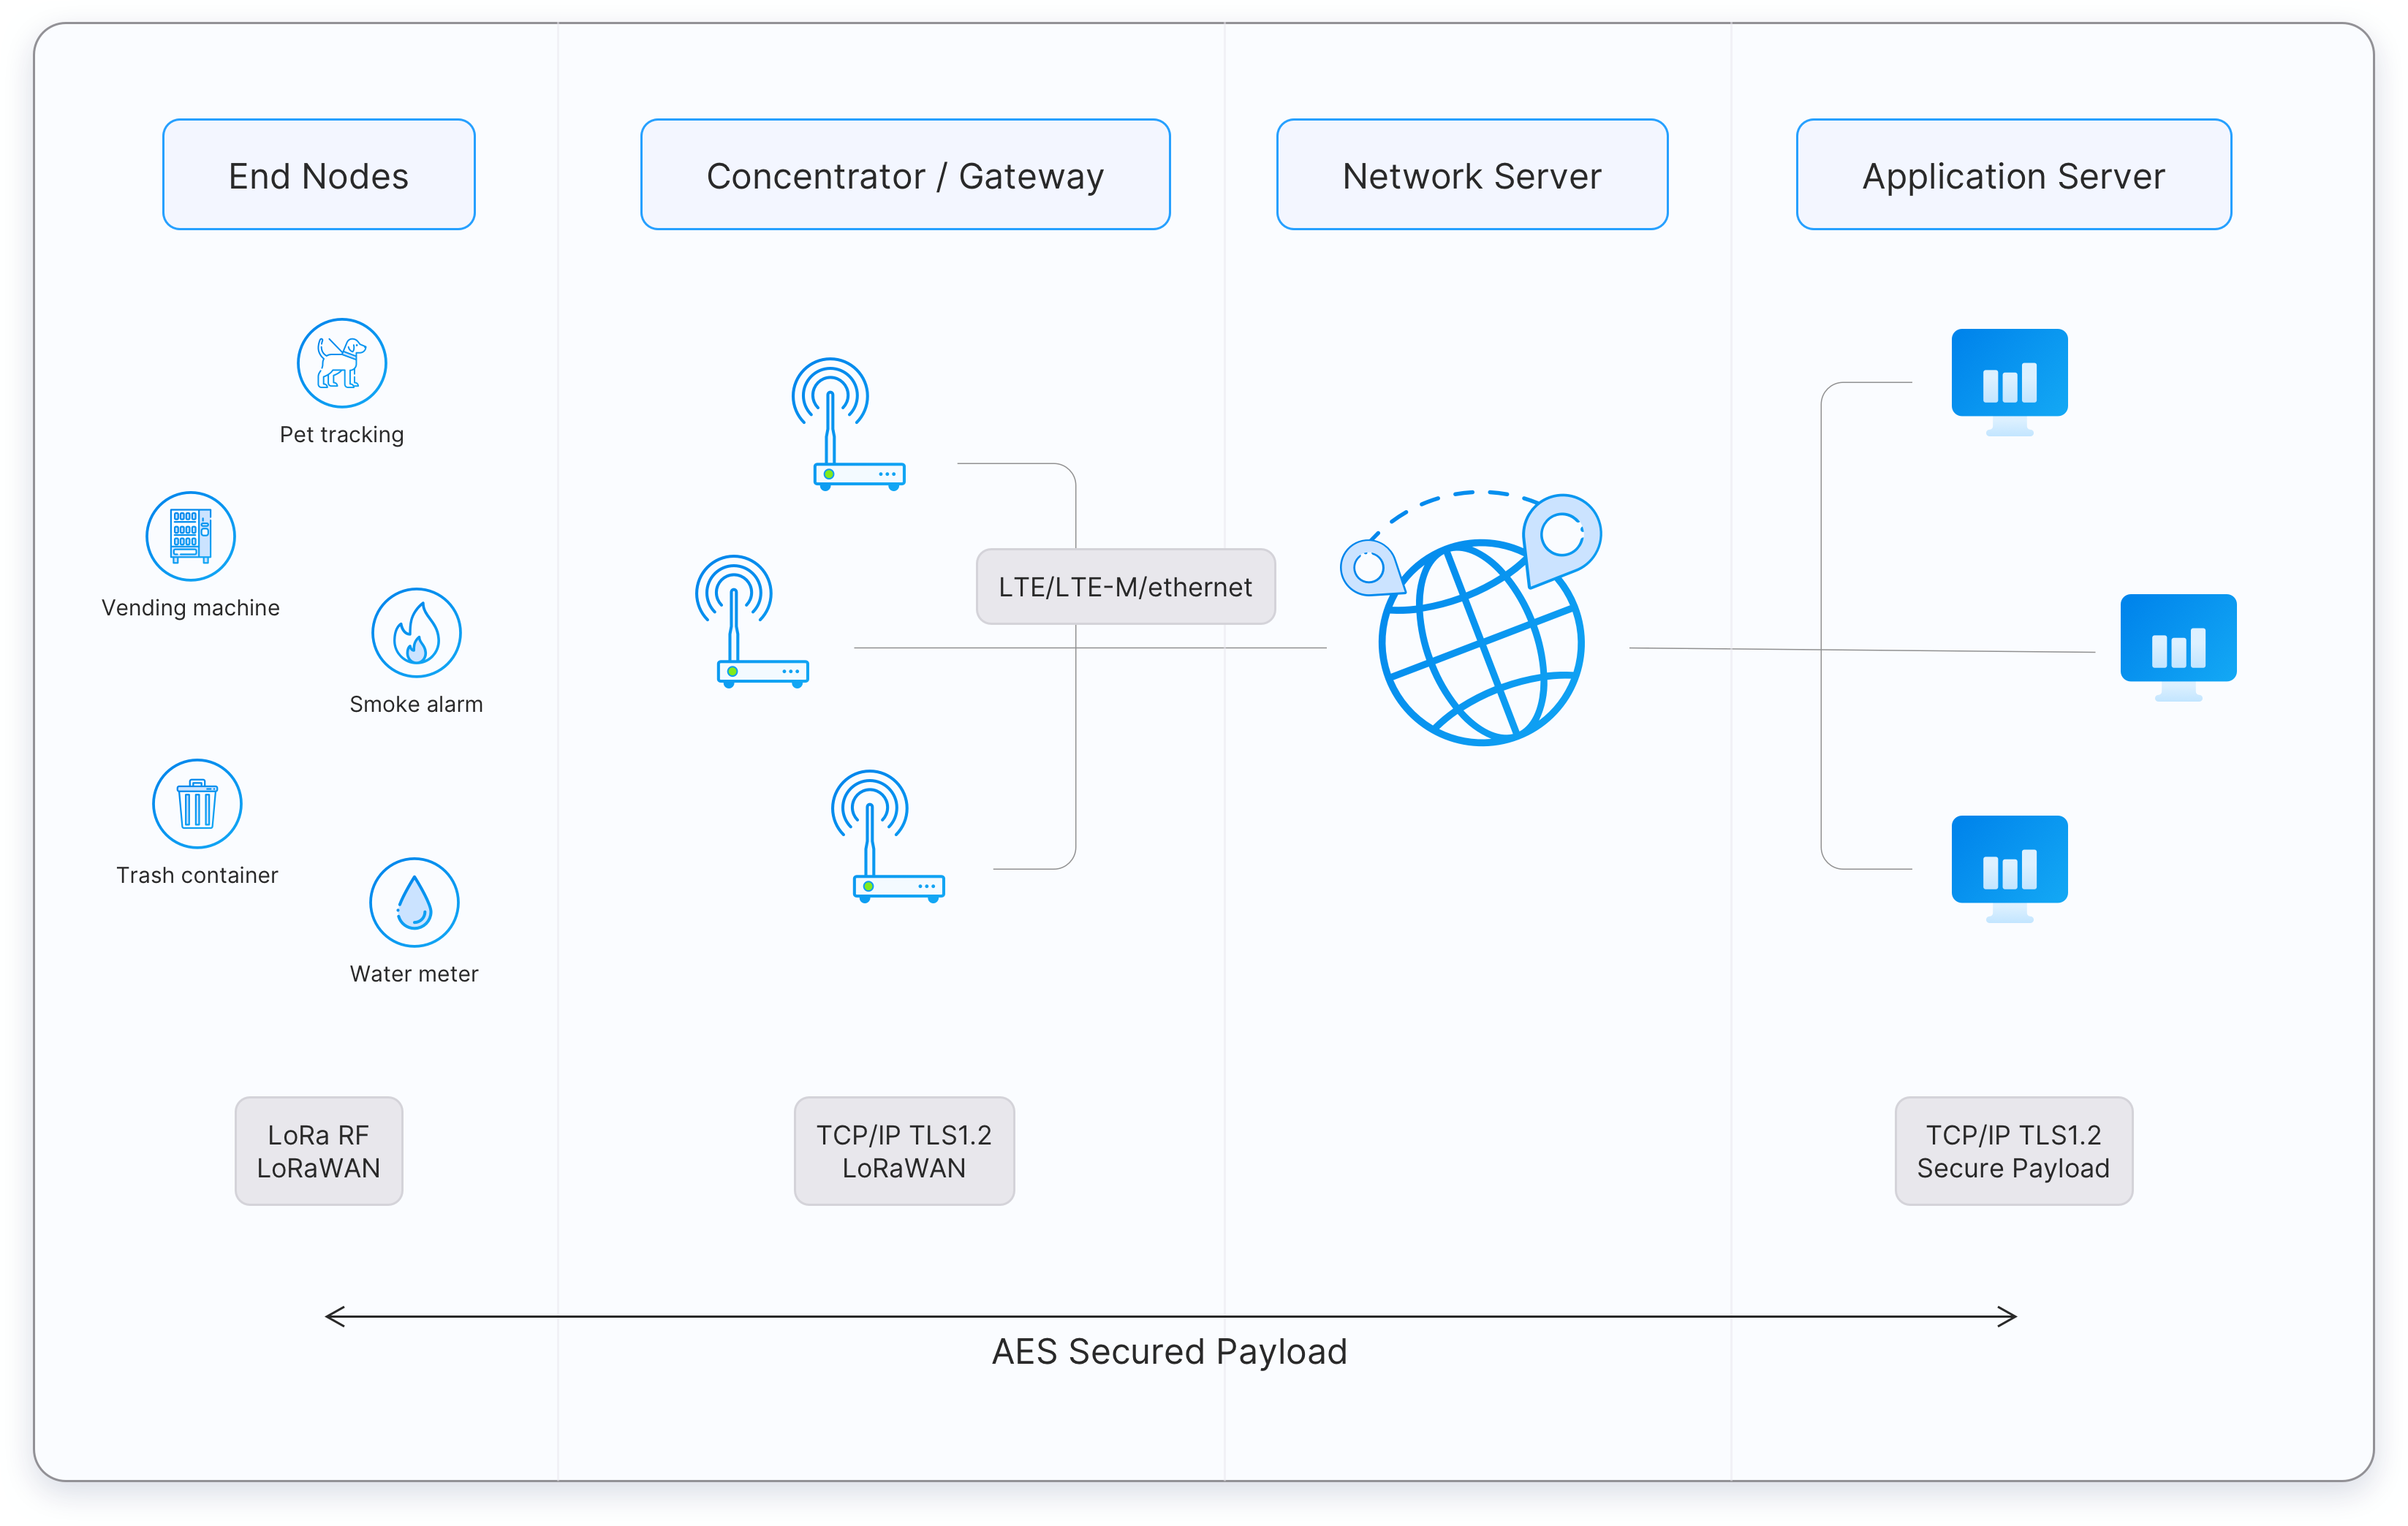
\includegraphics[width=0.8\textwidth]{figures/architecture_ttn.png}
    \caption{LoRaWAN Network Architecture}
    \label{fig:lora_architecture}
\end{figure}

LoRaWAN networks are deployed using a \emph{star-of-stars} topology.
Figure~\ref{fig:lora_architecture} shows the high-level architecture of a LoRaWAN network and its main components.
A typical LoRaWAN deployment comprises the following functional elements:

\begin{enumerate}
    \item \textbf{End Devices}: Sensors or actuators that transmit or receive LoRa-modulated wireless messages via gateways.
    \item \textbf{Gateways}: Multi-channel radio receivers that forward messages between end devices and the Network Server.
    \item \textbf{Network Server}: Centralized software responsible for managing network-level operations.
    \item \textbf{Application Servers}: Software components that process application-specific data securely.
    \item \textbf{Join Server}: Dedicated entity that handles secure device activation and key derivation (not always depicted in high-level diagrams).
\end{enumerate}

End devices communicate with all gateways within radio range. Gateways, in turn, are connected to the Network Server via backhaul links (e.g., Ethernet, cellular, or Wi-Fi). The medium access mechanism is based on an ALOHA-type protocol; thus, end devices do not establish persistent associations with specific gateways. Uplink messages may be received by multiple gateways simultaneously. The Network Server performs \emph{message deduplication} by retaining only one instance of each unique message and discarding redundant copies.

\subsection{End Devices}
\begin{figure}
    \centering
    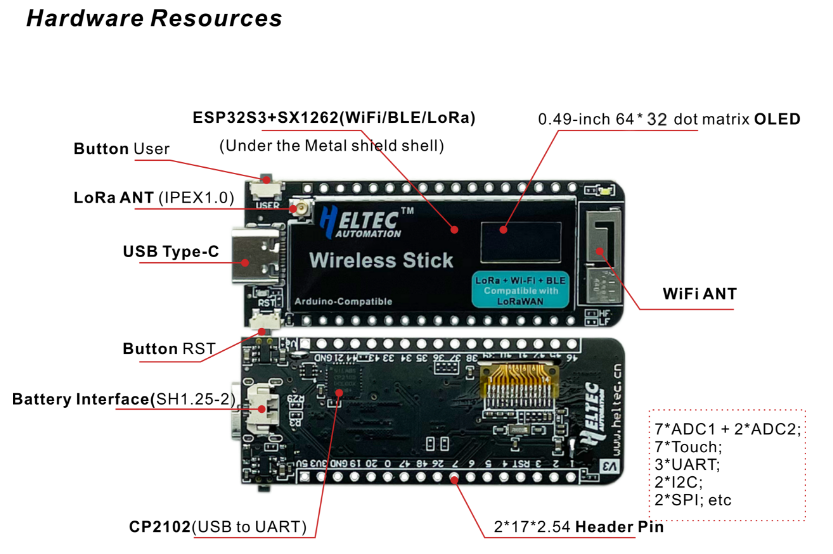
\includegraphics[width=0.6\textwidth]{figures/stick_v3.png}
    \caption{Heltec stick V3 LoRaWAN End Device}
    \label{fig:lora_end_device}
\end{figure}

A LoRaWAN end device is typically a low-power sensor, actuator, or a combination of both, often powered by batteries with lifespans ranging from several months to over a decade. These devices interface with the network exclusively through LoRa-based RF communication. Common sensing modalities include temperature, humidity, motion, and environmental parameters. End devices operate under strict regulatory constraints regarding transmit power, duty cycle, and channel usage, which are region-specific and enforced by the LoRaWAN regional parameters specification.
Figure~\ref{fig:lora_end_device} shows an example of a LoRaWAN end device.

\subsection{Gateways}
\begin{figure}
    \centering
    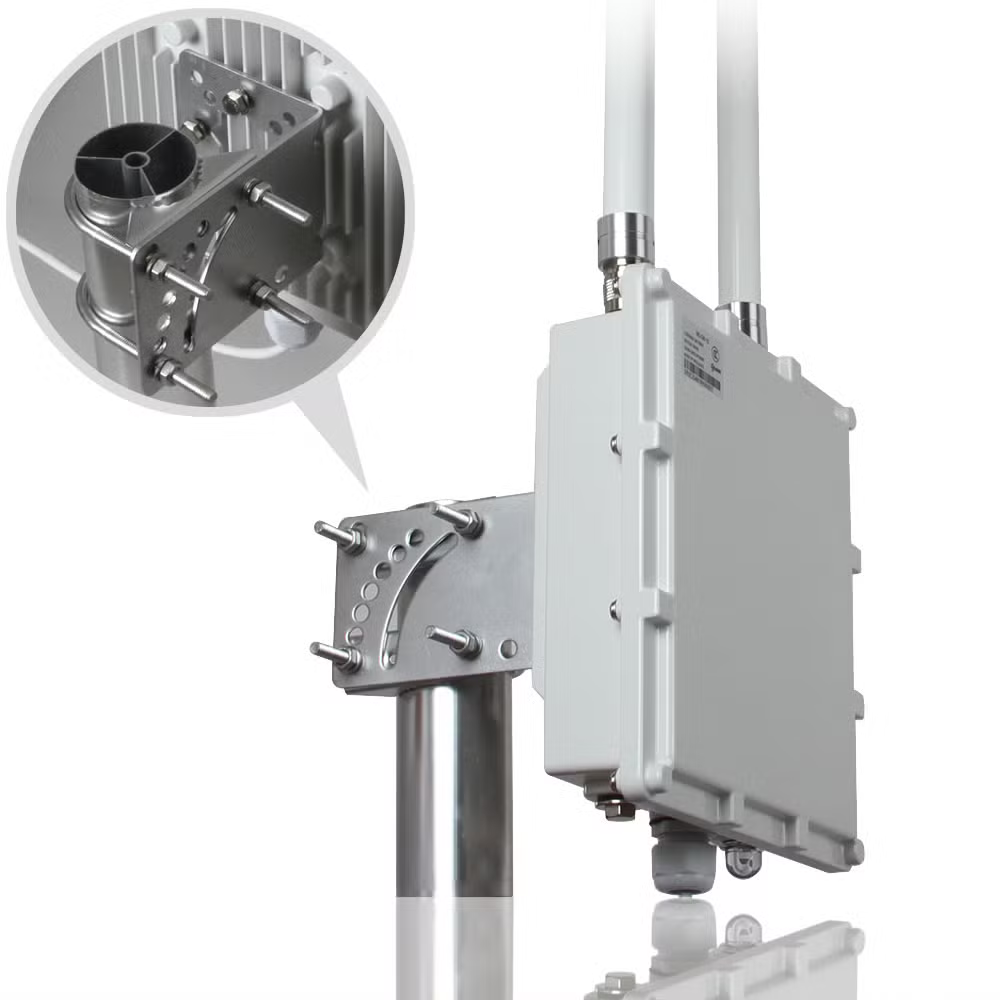
\includegraphics[width=0.6\textwidth]{figures/Ethernet-4G-Lorawan-Outdoor-Gateway-for-Remote-Street-Light-Management.png}
    \caption{LoRaWAN Gateway}
    \label{fig:lora_gateway}
\end{figure}
Gateways serve as transparent bridges between the RF layer and the IP-based core network. Each gateway is pre-configured to communicate with a designated Network Server. Upon receiving a LoRa-modulated frame, the gateway timestamps it, encapsulates it in a standardized protocol (e.g., LoRaWAN Backend Interfaces or Semtech UDP Packet Forwarder), and forwards it over the backhaul to the Network Server.

Figure~\ref{fig:lora_gateway} shows an example of a LoRaWAN gateway.

LoRaWAN gateways are broadly classified into two categories:

\begin{enumerate}
    \item \textbf{Indoor (Picocell) Gateways}:
          \begin{enumerate}
              \item Designed for deployment in residential, commercial, or industrial indoor environments.
              \item Typically feature integrated or short external antennas (e.g., pigtail connectors).
              \item Cost-effective and suitable for coverage in deep-indoor scenarios such as basements or multi-story buildings.
              \item Despite their form factor, some indoor gateways may receive signals from devices several kilometers away under favorable propagation conditions.
          \end{enumerate}

    \item \textbf{Outdoor (Macrocell) Gateways}:
          \begin{enumerate}
              \item Engineered for wide-area coverage in both urban and rural settings.
              \item Often mounted on elevated structures such as cellular towers, rooftops, or masts.
              \item Equipped with high-gain external antennas (e.g., fiberglass omnidirectional antennas) connected via coaxial cables.
              \item Exhibit superior receiver sensitivity compared to indoor counterparts.
              \item May support additional connectivity options (e.g., 3G/4G, GPS) for synchronization and backhaul redundancy.
              \item With appropriate environmental enclosures and antenna modifications, certain indoor gateways can be repurposed for outdoor use.
          \end{enumerate}
\end{enumerate}

\subsection{Network Server}

The Network Server (NS) is the core orchestration component of the LoRaWAN infrastructure. It manages the network state, enforces protocol compliance, and ensures secure and efficient data routing. Key responsibilities include:

\begin{enumerate}
    \item Establishing end-to-end security through 128-bit AES encryption using session keys (NwkSKey for network layer, AppSKey for application layer).
    \item Validating the authenticity of end devices and the integrity of received messages.
    \item Performing deduplication of uplink messages received from multiple gateways.
    \item Selecting the optimal gateway for downlink transmission based on signal quality and timing.
    \item Executing Adaptive Data Rate (ADR) algorithms to dynamically adjust device data rates and transmit power for network efficiency.
    \item Verifying device addresses (DevAddr) and managing device sessions.
    \item Acknowledging confirmed uplink frames as per MAC layer requirements.
    \item Routing application payloads to the appropriate Application Server(s).
    \item Forwarding Join-Request and Join-Accept messages between end devices and the Join Server.
    \item Processing and responding to all MAC commands defined in the LoRaWAN specification.
\end{enumerate}

\subsection{Application Server}

The Application Server (AS) is responsible for handling application-layer logic. It receives decrypted application payloads from the Network Server, interprets the data according to domain-specific requirements, and may initiate downlink communications by generating application payloads. These payloads are sent back to the target end device via the Network Server. A single LoRaWAN deployment may host multiple Application Servers, each serving distinct use cases or tenants. Advanced analytics, including machine learning and artificial intelligence techniques, are often applied to the collected data to derive actionable insights and support decision-making.

\subsection{Join Server}

The Join Server (JS) is a security-critical component introduced in LoRaWAN 1.1 and also supported in LoRaWAN 1.0.4 for enhanced security. Its primary functions are:

\begin{enumerate}
    \item Secure storage of root keys (e.g., AppKey in LoRaWAN 1.0, or AppKey and NwkKey in LoRaWAN 1.1).
    \item Processing Join-Request messages initiated by end devices during Over-the-Air Activation (OTAA).
    \item Deriving session keys (NwkSKey and AppSKey) upon successful authentication.
    \item Securely distributing NwkSKey to the Network Server and AppSKey to the Application Server.
\end{enumerate}

This separation of key management enhances security by ensuring that no single entity possesses both network and application session keys, thereby enforcing a principle of least privilege and enabling secure multi-tenant deployments.


\section{Regional Parameters}

LoRaWAN operates within globally available unlicensed Industrial, Scientific, and Medical (ISM) radio spectrum bands. Similar to Wi-Fi in the 2.4\,GHz and 5\,GHz bands, LoRaWAN enables deployment without requiring individual spectrum licensing. However, due to the use of lower frequencies—typically between 433\,MHz and 928\,MHz—LoRaWAN transmissions achieve longer range but are subject to stricter, country-specific regulatory constraints. To reconcile global interoperability with local compliance, the LoRa Alliance has defined standardized \emph{Regional Parameters} that specify region-specific physical and MAC layer configurations.

These Regional Parameters establish a common technical baseline for each regulatory domain but do not exhaustively define all operational details. Network operators may implement additional channels or policies beyond the specification, often referred to as \emph{Other} parameters. In some jurisdictions, multiple frequency plans are permissible; for instance, in the Netherlands, both EU863–870 and EU433 bands are authorized for LoRaWAN use.

The Regional Parameters encompass:
\begin{enumerate}
    \item Physical layer specifications, including:
          \begin{enumerate}
              \item Frequency (channel) plans
              \item Mandatory channels for network join
              \item Allowed data rates and spreading factors
              \item Transmit power limits (EIRP)
          \end{enumerate}
    \item MAC layer constraints, such as:
          \begin{enumerate}
              \item Maximum payload size per data rate
              \item Receive window timing and frequencies
              \item Duty cycle and dwell time limitations (where applicable)
          \end{enumerate}
\end{enumerate}

The official Regional Parameters document (RP002-1.0.4) defines thirteen distinct frequency plans, each assigned a unique Plan ID and common name, as summarized below.

\subsection{Frequency Plans}

\begin{enumerate}
    \item Plan ID 1: EU863–870 (common name: EU868)
    \item Plan ID 2: US902–928 (common name: US915)
    \item Plan ID 3: CN779–787 (common name: CN779)
    \item Plan ID 4: EU433 (common name: EU433)
    \item Plan ID 5: AU915–928 (common name: AU915)
    \item Plan ID 6: CN470–510 (common name: CN470)
    \item Plan ID 7: AS923-1 (common name: AS923)
    \item Plan ID 8: AS923-2 (common name: AS923-2)
    \item Plan ID 9: AS923-3 (common name: AS923-3)
    \item Plan ID 10: KR920–923 (common name: KR920)
    \item Plan ID 11: IN865–867 (common name: IN865)
    \item Plan ID 12: RU864–870 (common name: RU864)
    \item Plan ID 13: AS923-4 (common name: AS923-4)
\end{enumerate}

Each plan corresponds to one or more countries, as detailed in the LoRa Alliance’s Country Cross Reference Table. While comprehensive knowledge of all plans is not required, the EU863–870 and US902–928 bands are emphasized in certification contexts due to their widespread adoption.

\subsection{Default Settings for All Regions}

Certain timing and operational parameters are recommended uniformly across all regional implementations to ensure baseline interoperability. These default values are as follows:

\begin{enumerate}
    \item \textbf{RECEIVE\_DELAY1 (RX1 Delay)}: 1 second
    \item \textbf{RECEIVE\_DELAY2 (RX2 Delay)}: 2 seconds (defined as RX1 Delay + 1 second)
    \item \textbf{JOIN\_ACCEPT\_DELAY1}: 5 seconds
    \item \textbf{JOIN\_ACCEPT\_DELAY2}: 6 seconds
\end{enumerate}

These defaults may be overridden via MAC commands (e.g., \texttt{RXTimingSetupReq}) or during device provisioning, but deviations must be communicated to the Network Server during commissioning. The Network Server may reject non-standard timing configurations to maintain network integrity.

\subsection{Indonesia: AS923-2 Band}
\label{subsec:indonesia_as923}

In Indonesia, LoRaWAN operation is regulated under the \textbf{AS923-2} frequency plan, which is a variant of the broader AS923 regional specification defined in the LoRaWAN Regional Parameters document RP002-1.0.4. This plan accommodates the specific sub-band allocated by Indonesian regulatory authorities, namely the \textbf{920–923 MHz} ISM band.

The AS923 regional framework employs a frequency offset mechanism to support multiple national implementations using a common base specification. For Indonesia, the plan is designated as \textbf{AS923-2}, corresponding to a frequency offset of:

\begin{enumerate}
    \item \texttt{AS923\_FREQ\_OFFSET} = \texttt{0xFFFFB9B0} (32-bit signed integer)
    \item \texttt{AS923\_FREQ\_OFFSET\_HZ} = $-1.80$~MHz
\end{enumerate}

This offset shifts the nominal AS923 default channels from 923.2/923.4~MHz down to \textbf{921.4~MHz} and \textbf{921.6~MHz}, which constitute the mandatory default channels for all AS923-2 end-devices in Indonesia.

\begin{enumerate}
    \item \textbf{Default and Join Channels}:
          Every end-device must implement the following two default channels for both normal operation and Join-Request transmissions:
    \item Uplink/Downlink: 921.4~MHz (DR2–DR5)
    \item Uplink/Downlink: 921.6~MHz (DR2–DR5)
          These channels use LoRa modulation with 125~kHz bandwidth. The Join-Request data rate is restricted to DR2–DR5 (SF10–SF7) to ensure compatibility with the 400~ms dwell time limitation enforced in many AS923 jurisdictions until otherwise configured by the network.

    \item \textbf{Data Rate and TXPower Encoding}:
          The supported data rates are:
    \item DR0–DR5 (minimum for certification)
    \item DR0–DR7 (full optional support, including DR6: LoRa SF7/250~kHz and DR7: FSK 50~kbps)
          The maximum EIRP is \textbf{+16 dBm}. TXPower levels are defined relative to this maximum in 2~dB steps (TXPower 0 = +16 dBm, TXPower 1 = +14 dBm, etc.).

    \item \textbf{Dwell Time and Regulatory Compliance}:
          AS923-2 devices in Indonesia must support the \texttt{TxParamSetupReq} MAC command to receive dwell time configuration from the Network Server. By default, devices assume \texttt{UplinkDwellTime} = 1 (400~ms limit) until explicitly reconfigured. Downlink dwell time is always set to 0 (no restriction).

    \item \textbf{Receive Windows}:
    \item RX1 uses the same channel as the uplink. The downlink data rate is determined by the uplink DR and RX1DROffset (0–7).
    \item RX2 uses a fixed frequency of \textbf{921.4~MHz} (i.e., 923.2~MHz + \texttt{AS923\_FREQ\_OFFSET\_HZ}) with DR2 (SF10, 125~kHz).

    \item \textbf{Channel Plan Flexibility}:
          While only two default channels are mandated, end-devices must support a channel data structure for at least 24 channels. Additional channels may be configured via the CFList in the Join-Accept message or through MAC commands (e.g., \texttt{NewChannelReq}, \texttt{LinkADRReq}).

    \item \textbf{Listen-Before-Talk (LBT)}:
          Although not explicitly mandated for Indonesia in RP002-1.0.4, AS923 devices operating in regions with LBT requirements (e.g., Japan) must comply with ARIB STD-T108. Device manufacturers targeting Indonesia should verify current local regulations, as spectrum management policies may evolve.
\end{enumerate}

In summary, LoRaWAN deployments in Indonesia must adhere to the AS923-2 profile, which ensures regulatory compliance while maintaining interoperability within the broader AS923 ecosystem. Network operators and device vendors should configure frequency offsets and dwell time parameters appropriately during commissioning to guarantee correct operation.


\section{LoRaWAN Relay}
\begin{figure}
    \centering
    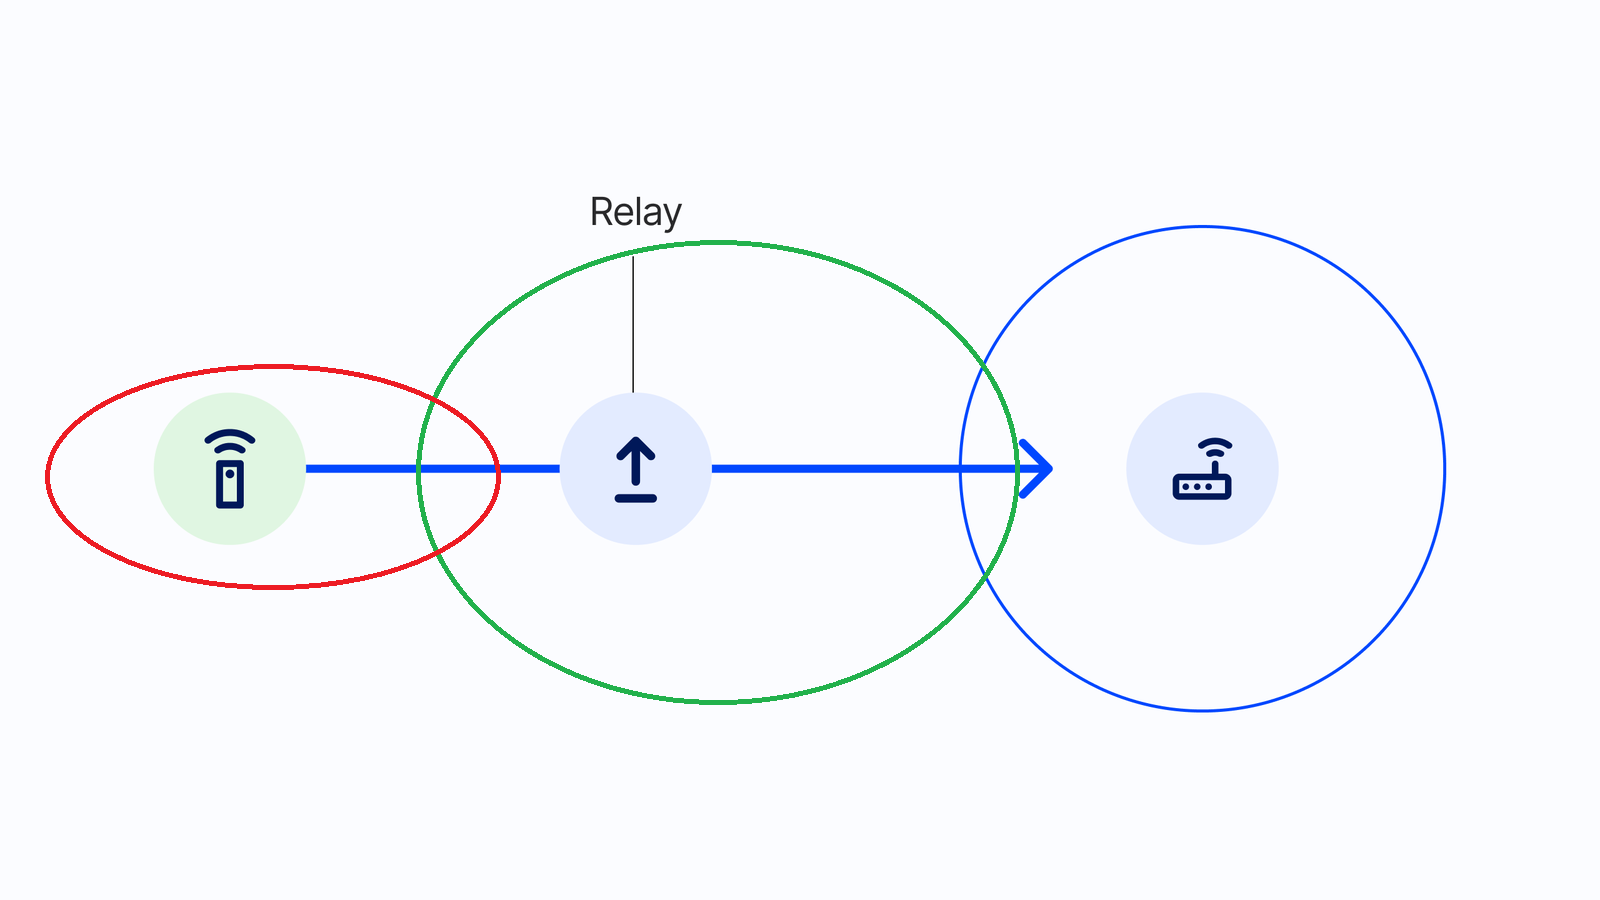
\includegraphics[width=0.8\textwidth]{figures/relay-placement.png}
    \caption{LoRaWAN Relay Architecture}
    \label{fig:lora_relay}
\end{figure}

LoRaWAN relays provide a cost-effective solution for extending network coverage in scenarios where direct communication between end devices and gateways is impaired due to excessive distance, physical obstructions, or signal attenuation. Relays operate as low-power, low-cost intermediaries that forward messages between end devices and the LoRaWAN infrastructure. From the perspective of the Network Server, a relay is functionally indistinguishable from a standard end device.
Figure~\ref{fig:lora_relay} illustrates the architecture of a LoRaWAN relay system.

\subsection{Relay Placement Strategy}

The deployment of a relay is economically justified when only a limited number of end devices experience connectivity issues. In contrast, if coverage deficiencies affect a large portion of the network, the installation of an additional gateway is typically more appropriate.

\subsection{Relay Requirements}

The functional and technical requirements for LoRaWAN relays are formally defined in the \emph{LoRaWAN\textsuperscript{\textregistered} Relay Specification} (TS011-1.0.0). Key implementation prerequisites include:

\begin{enumerate}
    \item The end device must implement:
          \begin{enumerate}
              \item The LoRaWAN MAC Layer Specification (TS001) version 1.0.4.
              \item The Regional Parameters Specification RP2-1.0.3.
              \item The LoRa Basics Modem firmware (experimental release available from Semtech).
          \end{enumerate}

    \item The end device hardware must incorporate one of the following sub-GHz LoRa transceivers:
          \begin{enumerate}
              \item SX1261/2
              \item LR1110
              \item LR1120
              \item LR1121
          \end{enumerate}

    \item The LoRaWAN Network Server (e.g., The Things Stack) must support the relay specification.

    \item Gateways require no modifications or firmware updates to support relay functionality.
\end{enumerate}

\subsection{Relay Operation}

Communication between an end device and the Network Server via a relay follows a structured sequence:

\begin{enumerate}
    \item Prior to communication, the end device and relay are pre-configured with shared channel parameters (frequency, data rate) for their direct link.

    \item To initiate communication, the end device transmits a \emph{Wake-on-Radio} (WOR) frame. This frame serves two purposes:
          \begin{enumerate}
              \item It wakes the relay from sleep mode.
              \item It conveys the radio parameters (frequency and data rate) for the subsequent uplink transmission.
          \end{enumerate}

    \item Two types of WOR frames are defined, distinguishable by payload content:
          \begin{enumerate}
              \item Relay Join-Request
              \item Relay Uplink (Class A uplink)
          \end{enumerate}

    \item The relay operates in a low-power sleep state and periodically performs \emph{Channel Activity Detection} (CAD) to monitor for incoming WOR frames. Key timing parameters include:
          \begin{enumerate}
              \item CAD duration: 25 ms to 1 s (default configuration dependent).
              \item CAD periodicity: interval between consecutive CAD operations.
              \item WOR preamble length: up to 1 s, ensuring high detection probability during brief CAD windows.
          \end{enumerate}

    \item Upon detecting LoRa activity during CAD, the relay transitions to receive mode after a \emph{CadToRx} delay. If the demodulated WOR frame is valid, the relay responds with a \emph{WOR-ACK} frame containing:
          \begin{enumerate}
              \item \texttt{CadToRx}: delay from CAD detection to reception readiness.
              \item \texttt{Forward}: relay forwarding capability status.
              \item \texttt{RelayDataRate}: data rate for upstream forwarding to the Network Server.
              \item \texttt{XTALAccuracy}: crystal oscillator accuracy of the relay.
              \item \texttt{CADPeriodicity}: interval between CAD scans.
              \item \texttt{TOffset}: time between CAD start and end of WOR preamble reception.
          \end{enumerate}

    \item The end device uses the WOR-ACK parameters to synchronize subsequent transmissions with the relay.

    \item The end device then transmits its LoRaWAN uplink frame. The relay receives this frame, prepends a 6-byte metadata header, and encapsulates the result as a \emph{Relay Uplink FRMPayload}. This payload is transmitted to the Network Server using FPort 226.

    \item Downlink messages from the Network Server (FPort 226) are received by the relay in RX1 or RX2 windows. The relay extracts the original payload and forwards it to the end device during the dedicated \emph{Relay Receive} (RXR) window.
\end{enumerate}

\subsection{Regional Parameters for Relays}

Relay-specific physical layer parameters are defined per regional band. Examples include:

\begin{enumerate}
    \item \textbf{EU868 (EU863–870 MHz)}:
          \begin{enumerate}
              \item WOR channels (end device $\rightarrow$ relay):
                    \begin{enumerate}
                        \item Channel 0: 856.1 MHz
                        \item Channel 1: 865.5 MHz
                    \end{enumerate}
              \item WOR-ACK channels (relay $\rightarrow$ end device):
                    \begin{enumerate}
                        \item Channel 0: 865.3 MHz
                        \item Channel 1: 865.9 MHz
                    \end{enumerate}
              \item Bandwidth: 125 kHz
              \item Spreading Factor: SF9
          \end{enumerate}

    \item \textbf{US915 (US902–928 MHz)}:
          \begin{enumerate}
              \item WOR channels (end device $\rightarrow$ relay):
                    \begin{enumerate}
                        \item Channel 0: 916.7 MHz
                        \item Channel 1: 919.9 MHz
                    \end{enumerate}
              \item WOR-ACK channels (relay $\rightarrow$ end device):
                    \begin{enumerate}
                        \item Channel 0: 918.3 MHz
                        \item Channel 1: 918.3 MHz
                    \end{enumerate}
              \item Bandwidth: 500 kHz
              \item Spreading Factor: SF10
          \end{enumerate}

    \item For other regions (AU915, CN470, AS923, KR920, IN865, RU864), relay channel frequencies, bandwidths, and spreading factors are specified in the LoRaWAN Regional Parameters document RP002-1.0.4.
\end{enumerate}

\subsection{Security Model}

Relay communication employs a dedicated security framework to ensure integrity and confidentiality of WOR and WOR-ACK frames:

\begin{enumerate}
    \item Standard session keys (\texttt{AppSKey}, \texttt{NwkSKey}) are insufficient for securing relay control frames.

    \item A new root key, the \emph{Root Relay Session Key} (\texttt{RootWorSKey}), is derived by the end device:
          \begin{enumerate}
              \item From \texttt{NwkSKey} in LoRaWAN 1.0.x.
              \item From \texttt{NwkSEncKey} in LoRaWAN 1.1.x and later.
          \end{enumerate}

    \item The Network Server provisions the same \texttt{RootWorSKey} to the relay during commissioning.

    \item Both end device and relay independently derive two session keys from \texttt{RootWorSKey} and \texttt{DevAddr}:
          \begin{enumerate}
              \item \texttt{WorSIntKey}: used to compute and verify the Message Integrity Code (MIC) of WOR and WOR-ACK frames.
              \item \texttt{WorSEncKey}: used to encrypt and decrypt the payload of WOR and WOR-ACK frames.
          \end{enumerate}
\end{enumerate}

\section{Message Types}

LoRaWAN defines a structured set of message types to facilitate secure and efficient communication between end devices, gateways, and network entities. These messages transport both Medium Access Control (MAC) commands and application-layer data. Understanding message classification, structure, encryption, and integrity mechanisms is essential for interoperability and security compliance, particularly in LoRaWAN versions 1.0.x and 1.1.

\subsection{Uplink and Downlink Messages}

Messages in LoRaWAN are categorized by their direction of transmission:

\begin{enumerate}
    \item \textbf{Uplink messages}: Originating from end devices and relayed to the Network Server via one or more gateways. Depending on the destination, the Network Server forwards these messages to either the Application Server or the Join Server.
    \item \textbf{Downlink messages}: Sent by the Network Server to a specific end device and delivered through a single selected gateway. These may originate from the Network Server itself, the Application Server, or the Join Server.
\end{enumerate}

\subsection{MAC Message Types}

LoRaWAN specifies distinct MAC message types for network control and data transport. The following enumeration outlines the message types supported in LoRaWAN 1.0.x and 1.1:

\begin{enumerate}
    \item \textbf{Join-request}: An uplink message used during Over-the-Air Activation (OTAA) to initiate a session.
    \item \textbf{Join-accept}: A downlink response to a Join-request, providing session parameters.
    \item \textbf{Unconfirmed Data Up}: An uplink data frame that does not require acknowledgment.
    \item \textbf{Unconfirmed Data Down}: A downlink data frame that does not require acknowledgment.
    \item \textbf{Confirmed Data Up}: An uplink data frame that requires acknowledgment from the receiver.
    \item \textbf{Confirmed Data Down}: A downlink data frame that requires acknowledgment from the end device.
    \item \textbf{Rejoin-request} (LoRaWAN 1.1 only): An uplink message used to re-establish a session context without full reactivation; supports three subtypes (0, 1, 2).
    \item \textbf{Proprietary}: Reserved for vendor-specific extensions.
    \item \textbf{RFU} (LoRaWAN 1.0.x): Reserved for future use; repurposed as Rejoin-request in 1.1.
\end{enumerate}

\subsection{Join-Request, Rejoin-Request, and Join-Accept Messages}

\begin{enumerate}
    \item \textbf{Join-request}:
          \begin{enumerate}
              \item Initiated by the end device.
              \item In LoRaWAN 1.0.4 and earlier, forwarded by the Network Server to the Application Server.
              \item In LoRaWAN 1.1 and 1.0.4+, forwarded to the Join Server.
              \item Transmitted unencrypted.
          \end{enumerate}

    \item \textbf{Join-accept}:
          \begin{enumerate}
              \item Generated by the Join Server (1.1 and 1.0.4+) or Application Server (pre-1.0.4).
              \item Routed to the end device via the Network Server.
              \item Encryption key depends on LoRaWAN version and triggering message:
                    \begin{enumerate}
                        \item LoRaWAN 1.0: encrypted with \texttt{AppKey}.
                        \item LoRaWAN 1.1:
                        \item Triggered by Join-request: encrypted with \texttt{NwkKey}.
                        \item Triggered by Rejoin-request (Types 0, 1, 2): encrypted with \texttt{JSEncKey}.
                    \end{enumerate}
          \end{enumerate}

    \item \textbf{Rejoin-request} (LoRaWAN 1.1 only):
          \begin{enumerate}
              \item Initiated by the end device to refresh session keys or rejoin after roaming.
              \item Three types defined (0, 1, 2), differing in identifier scope (NetID vs. JoinEUI).
              \item Always responded to with a Join-accept message.
          \end{enumerate}
\end{enumerate}

\subsection{Data Messages}
\begin{figure}
    \centering
    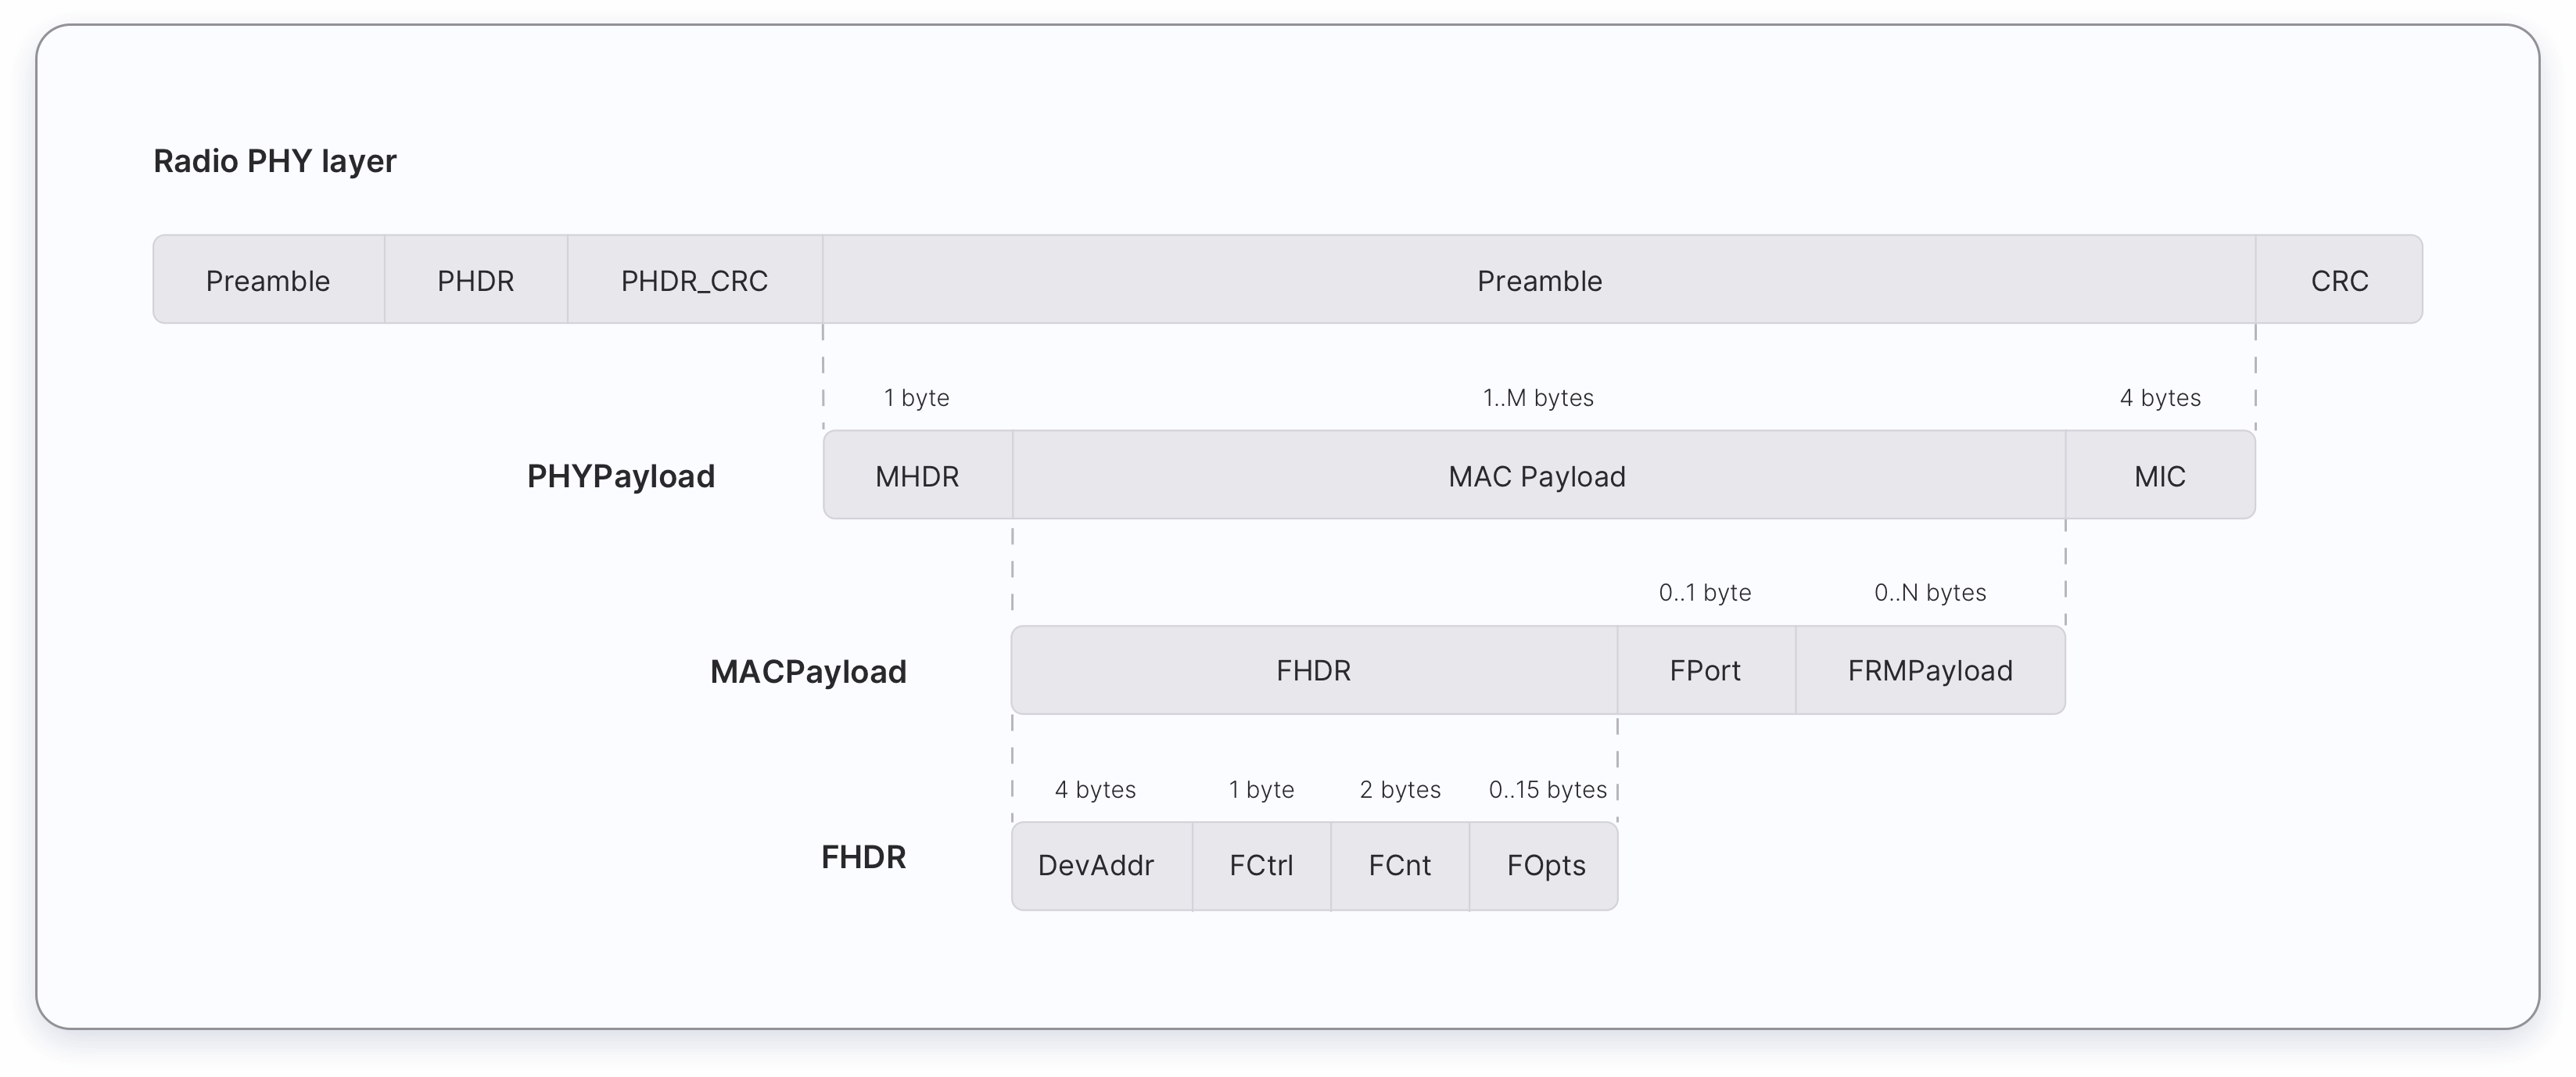
\includegraphics[width=0.8\textwidth]{figures/payload.png}
    \caption{LoRaWAN Data Message Structure}
    \label{fig:lora_data_message}
\end{figure}

Data messages transport application payloads and/or MAC commands. Four types exist, consistent across LoRaWAN 1.0.x and 1.1:
Figure~\ref{fig:lora_data_message} illustrates the structure of a LoRaWAN data message.
\begin{enumerate}
    \item Unconfirmed Data Up
    \item Unconfirmed Data Down
    \item Confirmed Data Up
    \item Confirmed Data Down
\end{enumerate}

A data message comprises a MAC payload structured as follows:

\begin{enumerate}
    \item \textbf{Frame Header (FHDR)}: 7–22 bytes, containing:
          \begin{enumerate}
              \item \texttt{DevAddr} (4 bytes)
              \item \texttt{FCtrl} (1 byte)
              \item \texttt{FCnt} (2 bytes)
              \item \texttt{FOpts} (0–15 bytes)
          \end{enumerate}
    \item \textbf{FPort} (0–1 byte, optional): Indicates content of FRMPayload.
    \item \textbf{FRMPayload} (0–N bytes, optional): Carries either MAC commands or application data.
\end{enumerate}

The maximum MAC payload length is region- and data rate-dependent, as defined in the Regional Parameters specification.

\subsection{Sending MAC Commands and Application-Specific Data}

MAC commands and application data are mutually exclusive within the FRMPayload field but may coexist in a message if MAC commands are placed in FOpts and application data in FRMPayload.

\begin{enumerate}
    \item \textbf{MAC commands in FOpts}:
          \begin{enumerate}
              \item Total length must not exceed 15 bytes.
              \item In LoRaWAN 1.0.x: transmitted unencrypted.
              \item In LoRaWAN 1.1: encrypted using \texttt{NwkSEncKey}.
          \end{enumerate}

    \item \textbf{MAC commands or application data in FRMPayload}:
          \begin{enumerate}
              \item Requires the presence of the FPort field.
              \item FPort interpretation:
                    \begin{enumerate}
                        \item \texttt{FPort = 0}: FRMPayload contains only MAC commands.
                        \item \texttt{FPort = 1–223}: FRMPayload contains application data.
                        \item \texttt{FPort = 224}: Reserved for LoRaWAN MAC layer test protocol.
                        \item \texttt{FPort = 255}: Reserved for Future Use (RFU).
                    \end{enumerate}
              \item Encryption of FRMPayload:
                    \begin{enumerate}
                        \item MAC commands (FPort = 0):
                        \item LoRaWAN 1.0.x: encrypted with \texttt{NwkSKey}.
                        \item LoRaWAN 1.1: encrypted with \texttt{NwkSEncKey}.
                        \item Application data (FPort = 1–223): encrypted with \texttt{AppSKey} in both versions.
                    \end{enumerate}
          \end{enumerate}
\end{enumerate}

\subsection{Message Integrity Code (MIC) Calculation}

The MIC ensures message authenticity and integrity. It is computed over specific fields and appended to the message. The fields and keys used depend on the LoRaWAN version and message type.

\begin{enumerate}
    \item \textbf{Fields used in MIC computation}:
          \begin{enumerate}
              \item LoRaWAN 1.0.x:
                    \begin{enumerate}
                        \item Join-request: \texttt{MHDR | AppEUI | DevEUI | DevNonce}
                        \item Join-accept: \texttt{MHDR | AppNonce | NetID | DevAddr | DLSettings | RxDelay | CFList}
                        \item Data messages (up/down): \texttt{MHDR | FHDR | FPort | FRMPayload}
                    \end{enumerate}
              \item LoRaWAN 1.1:
                    \begin{enumerate}
                        \item Join-request: \texttt{MHDR | JoinEUI | DevEUI | DevNonce}
                        \item Join-accept: \texttt{MHDR | JoinNonce | NetID | DevAddr | DLSettings | RxDelay | CFList}
                        \item Rejoin-request Type 0/2: \texttt{MHDR | Rejoin Type | NetID | DevEUI | RJcount0}
                        \item Rejoin-request Type 1: \texttt{MHDR | Rejoin Type | JoinEUI | DevEUI | RJcount1}
                        \item Data messages (up/down): \texttt{MHDR | FHDR | FPort | FRMPayload}
                    \end{enumerate}
          \end{enumerate}

    \item \textbf{Keys used for MIC computation}:
          \begin{enumerate}
              \item LoRaWAN 1.0.x:
                    \begin{enumerate}
                        \item Join-request: \texttt{AppKey}
                        \item Join-accept: \texttt{AppKey}
                        \item Uplink data: \texttt{NwkSKey}
                        \item Downlink data: \texttt{NwkSKey}
                    \end{enumerate}
              \item LoRaWAN 1.1:
                    \begin{enumerate}
                        \item Join-request: \texttt{NwkKey}
                        \item Join-accept: \texttt{JSIntKey}
                        \item Rejoin-request Type 0/2: \texttt{SNwkSIntKey}
                        \item Rejoin-request Type 1: \texttt{JSIntKey}
                        \item Uplink data: \texttt{FNwkSIntKey} (for MIC verification) and \texttt{SNwkSIntKey} (for generation in some contexts)
                        \item Downlink data: \texttt{SNwkSIntKey}
                    \end{enumerate}
              \item LoRaWAN 1.1 device operating with a 1.0.x Network Server:
                    \begin{enumerate}
                        \item Join-request: \texttt{NwkKey}
                        \item Join-accept: \texttt{NwkKey}
                        \item Uplink data: \texttt{FNwkSIntKey}
                        \item Downlink data: \texttt{FNwkSIntKey}
                    \end{enumerate}
          \end{enumerate}
\end{enumerate}


\section{Security}

LoRaWAN employs a robust security framework based on symmetric cryptography to ensure confidentiality, integrity, and authenticity of communications. The security model is built upon a set of 128-bit keys and utilizes the Advanced Encryption Standard (AES-128), consistent with cryptographic practices in standards such as IEEE 802.15.4.

\subsection{Security Keys}

The LoRaWAN 1.0 specification defines three primary cryptographic keys, each 128 bits in length:

\begin{enumerate}
    \item \textbf{AppKey} (Application Key): A root key used exclusively during the Over-the-Air Activation (OTAA) procedure to derive session keys. It is shared only between the end-device and the Join Server (or Application Server in pre-1.1 deployments).
    \item \textbf{NwkSKey} (Network Session Key): A session key used for securing communication between the end-device and the Network Server.
    \item \textbf{AppSKey} (Application Session Key): A session key used for end-to-end encryption of application-layer payloads between the end-device and the Application Server.
\end{enumerate}

\subsection{Session Keys}

Upon successful network activation—either via OTAA or pre-provisioned Activation-by-Personalization (ABP)—two session keys are established:

\begin{enumerate}
    \item The \textbf{Network Session Key (NwkSKey)} is used to:
          \begin{enumerate}
              \item Compute and verify the Message Integrity Code (MIC) of all MAC and data messages using AES-CMAC.
              \item Ensure message authenticity and prevent tampering.
              \item Assist the Network Server in mapping the non-unique device address (\texttt{DevAddr}) to the globally unique \texttt{DevEUI} and \texttt{AppEUI} identifiers.
          \end{enumerate}

    \item The \textbf{Application Session Key (AppSKey)} is used to:
          \begin{enumerate}
              \item Encrypt and decrypt the application payload (\texttt{FRMPayload}) of uplink and downlink messages.
              \item Provide end-to-end confidentiality between the end-device and the Application Server.
              \item Ensure that intermediate network entities (e.g., gateways, Network Server) cannot access application data.
          \end{enumerate}
\end{enumerate}

These session keys are unique per device and per session. In OTAA, keys are regenerated upon each join request. In ABP, keys remain static unless manually updated.

\subsection{Application Key}

The \textbf{Application Key (AppKey)} serves as the root secret for OTAA devices:

\begin{enumerate}
    \item It is never transmitted over the air.
    \item It is used during the join procedure to derive both \texttt{NwkSKey} and \texttt{AppSKey} through a key derivation function specified in the LoRaWAN MAC layer specification.
    \item In network deployments such as The Things Network, a default \texttt{AppKey} may be configured per application, or individual keys may be assigned per device for enhanced security.
\end{enumerate}

\subsection{Frame Counters}

To mitigate replay attacks—where an adversary captures and retransmits valid messages—LoRaWAN employs uplink and downlink frame counters:

\begin{enumerate}
    \item \texttt{FCntUp}: Incremented by the end-device for each uplink transmission.
    \item \texttt{FCntDown}: Incremented by the Network Server for each downlink transmission.
    \item Both counters are initialized to zero upon session establishment.
    \item The receiver (device or server) discards any message with a frame counter less than or equal to the last successfully received counter value.
    \item This mechanism ensures that each message is processed only once, even if intercepted and replayed.
\end{enumerate}

For ABP devices, frame counters are typically reset to zero on every power cycle or firmware update. Consequently, the Network Server will reject subsequent messages until the counter exceeds the previously recorded value. To avoid this during development, it is recommended to re-register ABP devices in the network server after each reset or to persist frame counters in non-volatile memory.

\subsection{Spread Spectrum and Security Considerations}

LoRa employs Chirp Spread Spectrum (CSS) modulation, a form of direct-sequence spread spectrum (DSSS). While spread spectrum techniques historically provided low probability of intercept (LPI) in military communications, LoRa’s use of CSS is primarily motivated by:

\begin{enumerate}
    \item Robustness against multipath fading and Doppler shifts.
    \item High link budget and long-range capability.
    \item Coexistence in dense spectral environments through processing gain.
\end{enumerate}

It should be emphasized that CSS in LoRaWAN does \emph{not} constitute a cryptographic security mechanism. Message confidentiality and integrity are solely ensured by the AES-based keying framework described above, not by the physical layer modulation. Therefore, reliance on spread spectrum for security against eavesdropping is unwarranted; cryptographic protections remain essential.


\section{Device Classes}

The LoRaWAN specification defines three device classes—Class A, Class B, and Class C—to accommodate varying application requirements in terms of power consumption, latency, and communication patterns. All LoRaWAN end-devices are required to implement Class A functionality. Class B and Class C are optional extensions that build upon Class A. All classes support bidirectional communication (uplink and downlink). During Firmware Updates Over-The-Air (FUOTA), devices must operate in either Class B or Class C to enable timely delivery of large firmware payloads.

It is important to note that end-devices cannot transmit uplink messages while receiving downlink messages due to half-duplex radio constraints.

\subsection{Class A}
\begin{figure}[htbp]
    \centering
    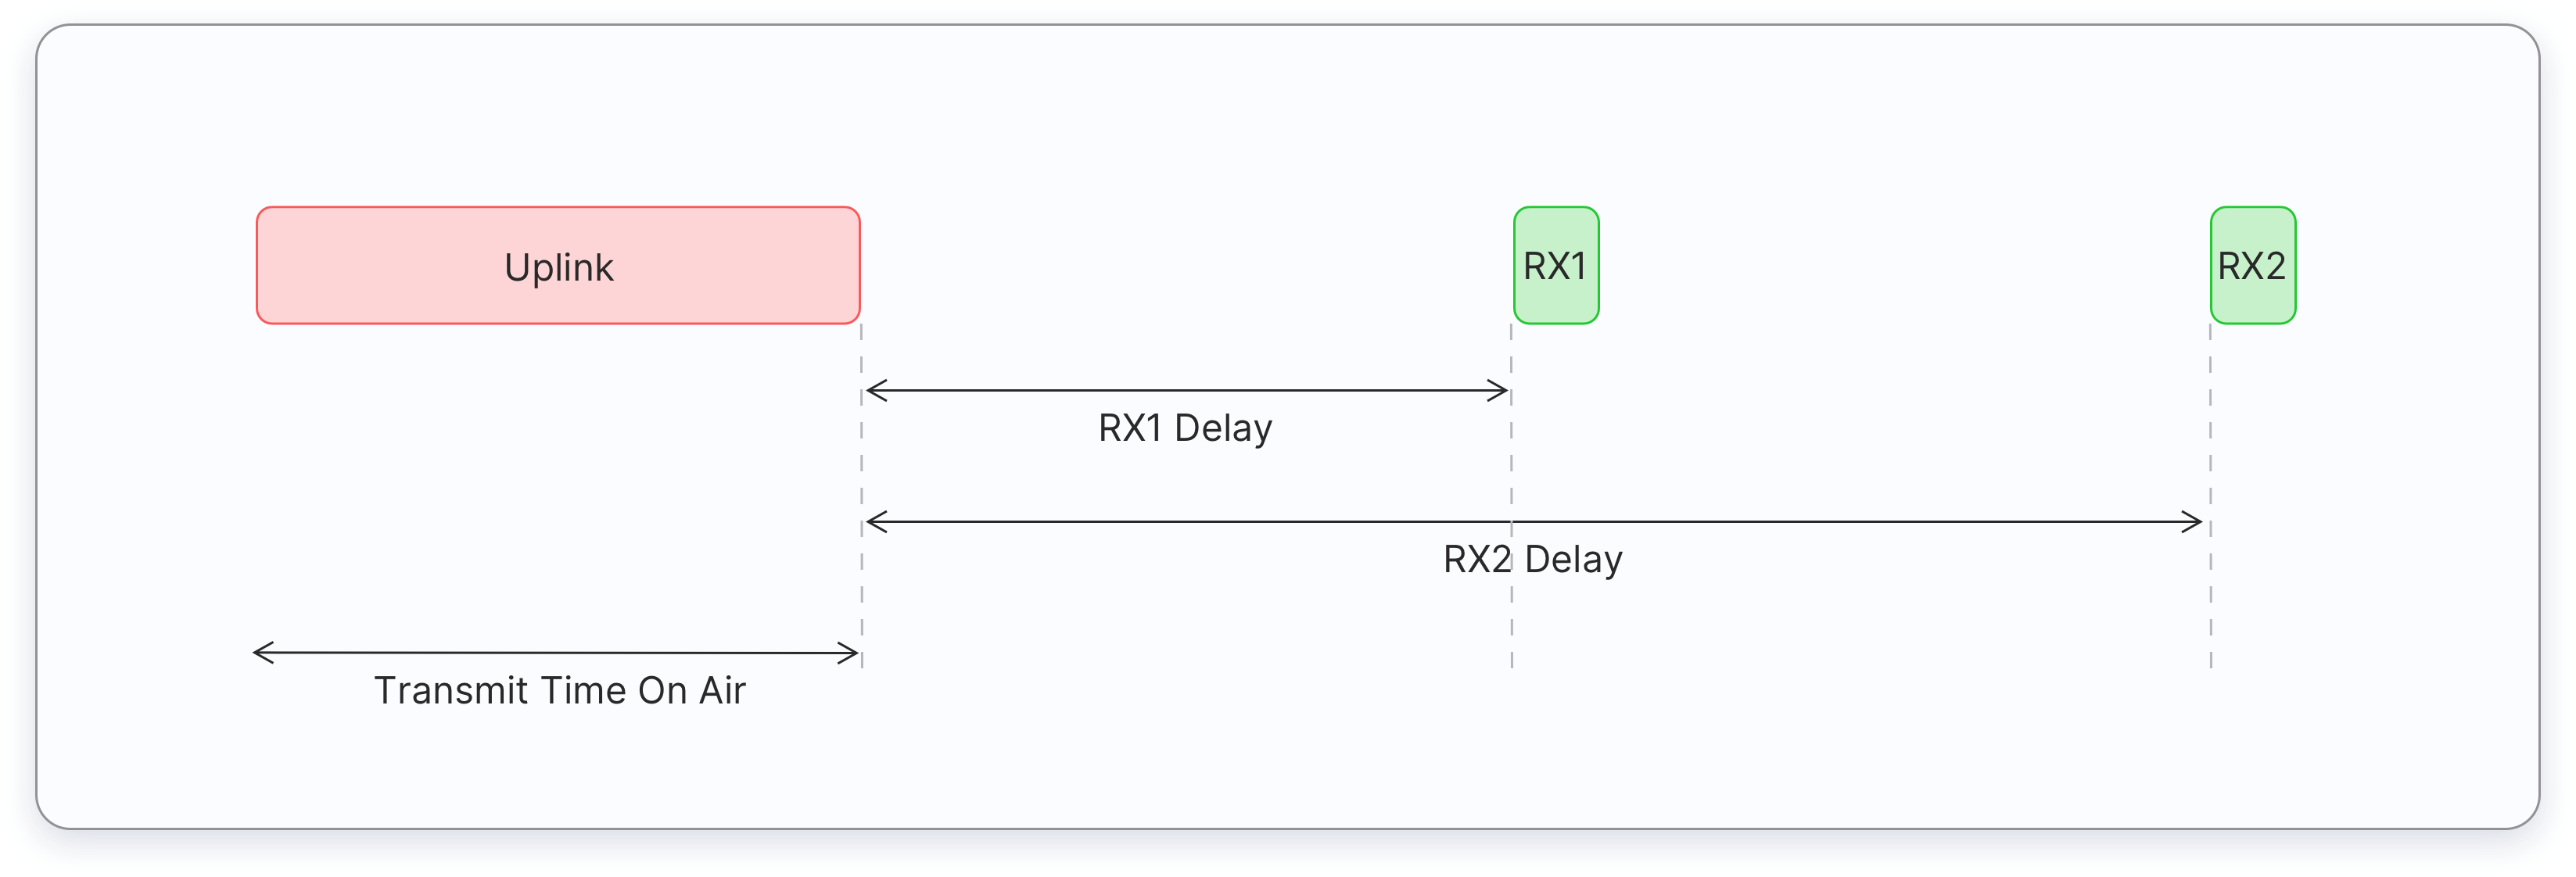
\includegraphics[width=0.8\textwidth]{figures/class-a.png}
    \caption{LoRaWAN Class A Operation}
    \label{fig:lora_class_a}
\end{figure}

\begin{figure}
    \centering
    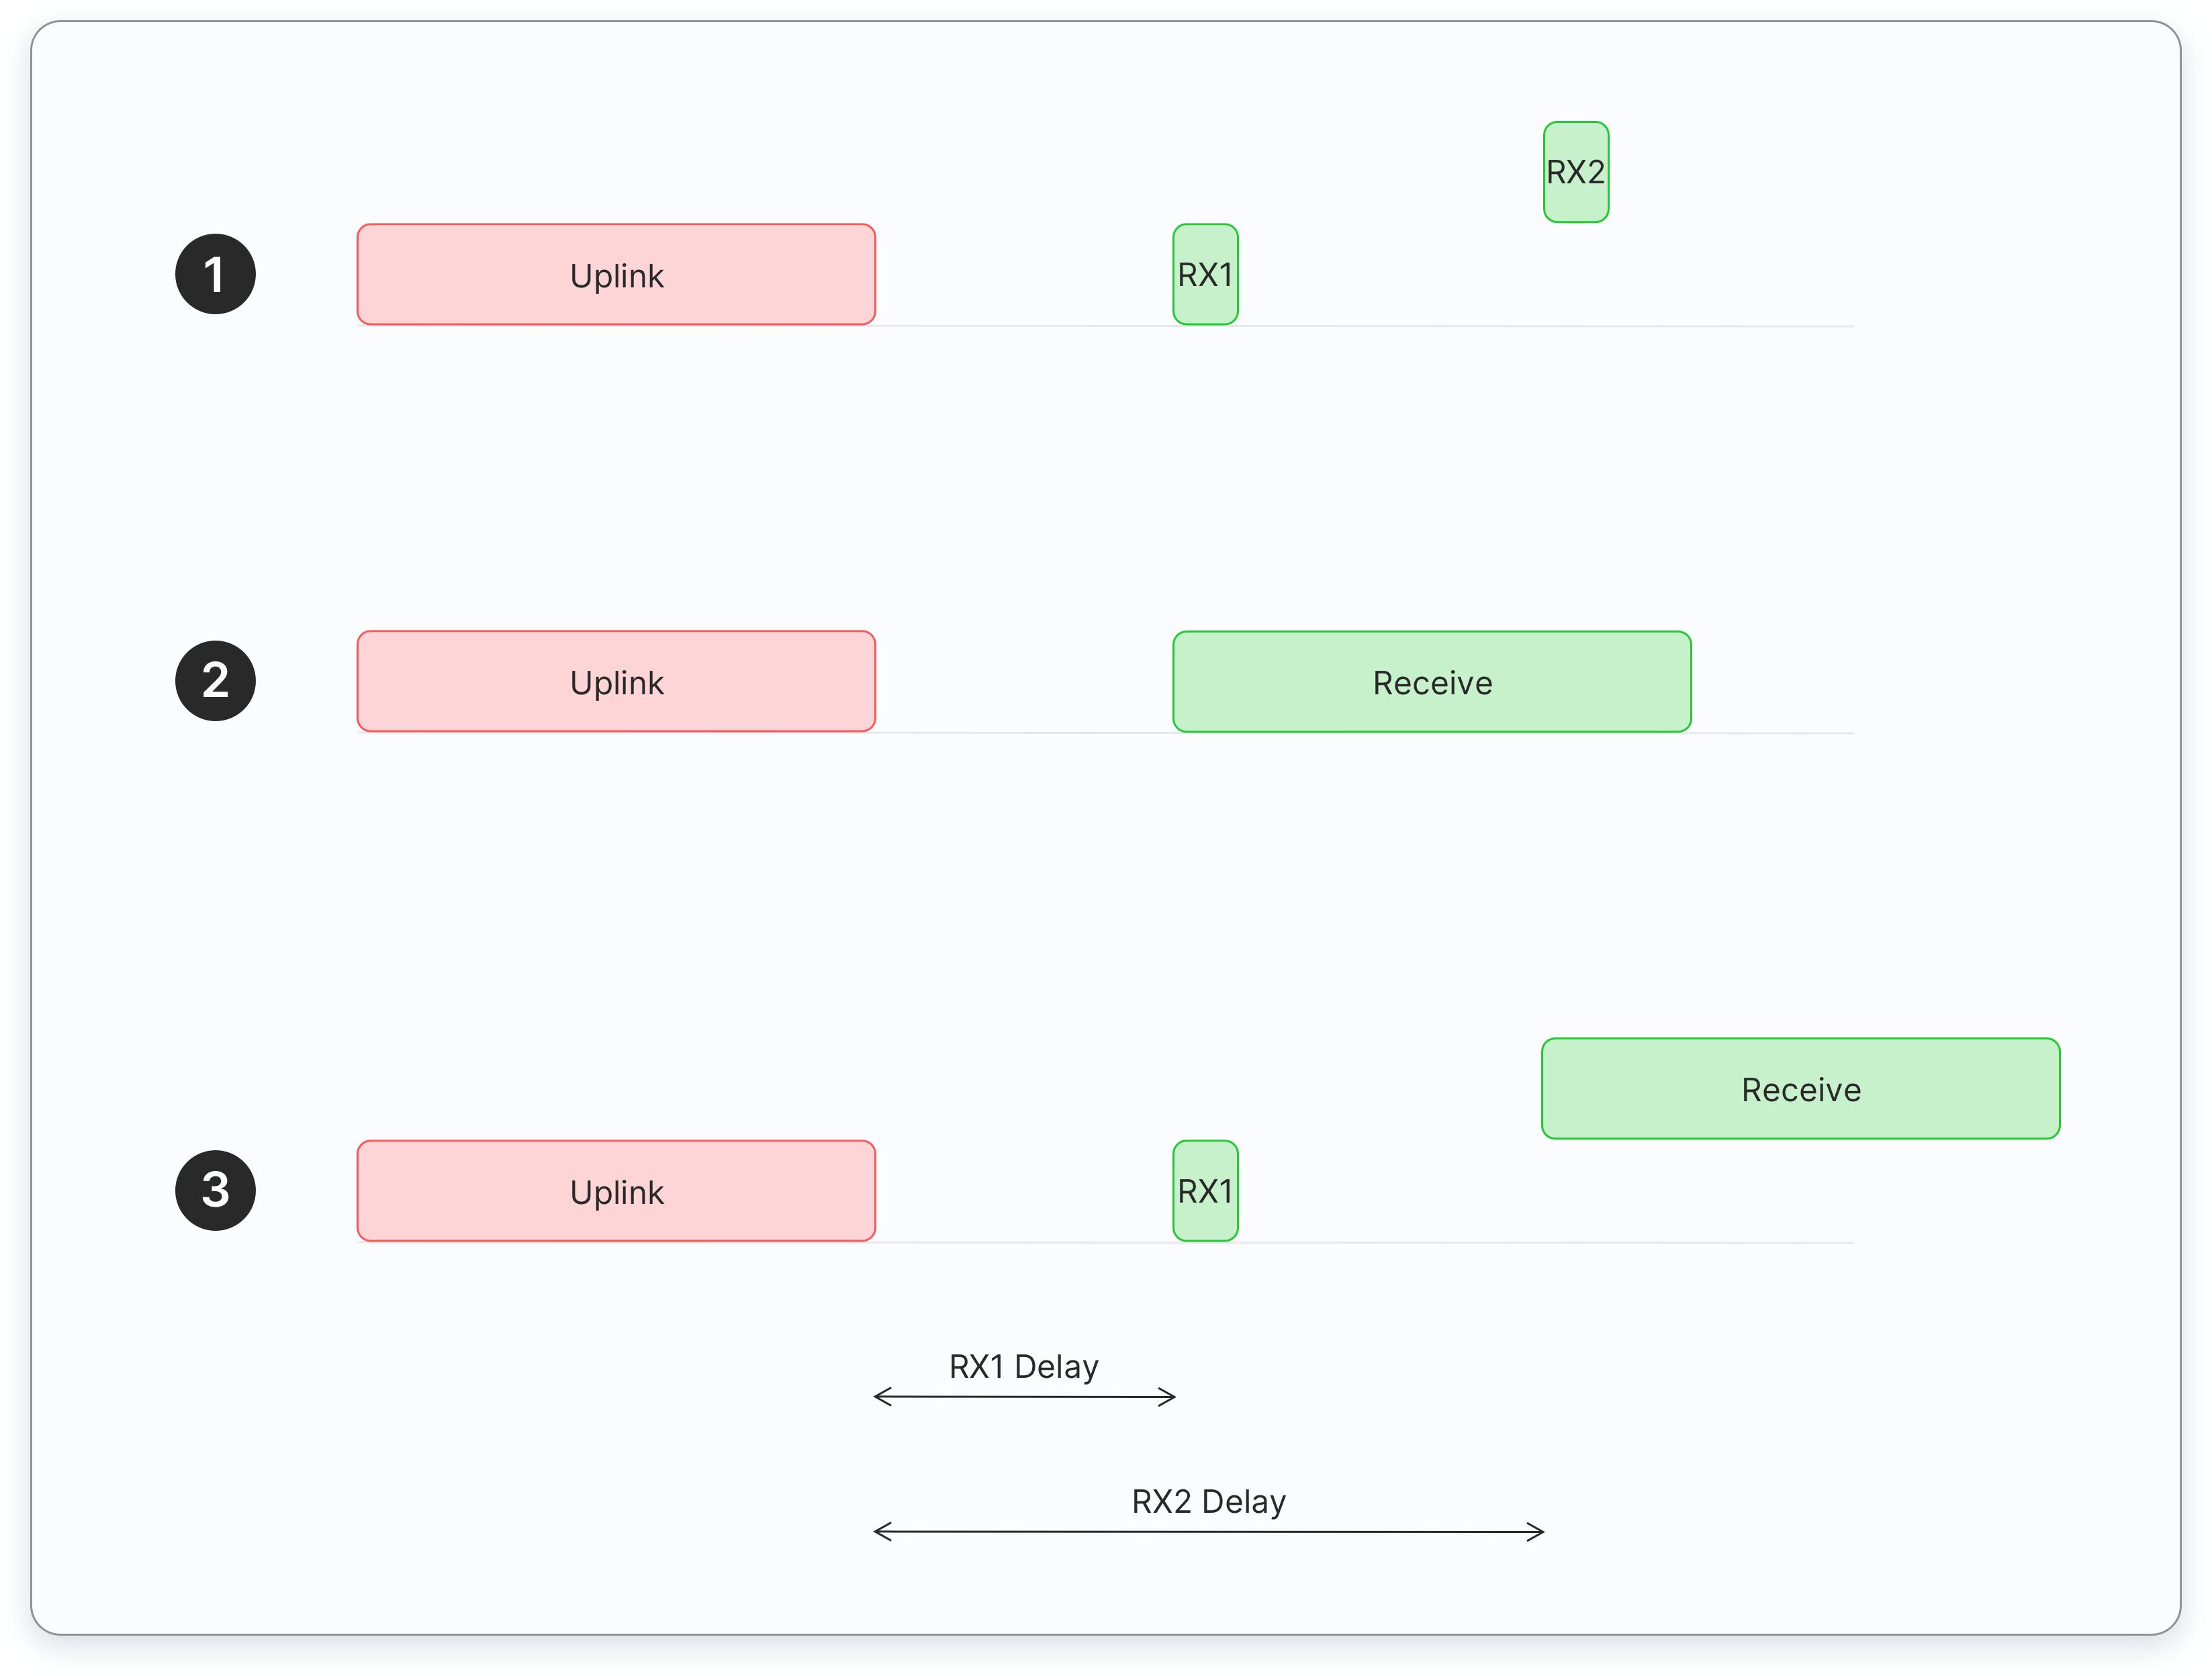
\includegraphics[width=0.8\textwidth]{figures/class-a-alt.png}
    \caption{LoRaWAN Class A Alternative Operation}
    \label{fig:lora_class_a_alt}
\end{figure}

Class A is the foundational and mandatory device class in LoRaWAN. Its design prioritizes ultra-low power consumption, making it suitable for battery-operated applications with infrequent communication needs.
Figures~\ref{fig:lora_class_a} and~\ref{fig:lora_class_a_alt} illustrate the timing of uplink and downlink transmissions in Class A devices.

\begin{enumerate}
    \item An end-device may initiate an uplink transmission at any time.
    \item Upon completion of an uplink transmission, the device opens two sequential receive windows:
          \begin{enumerate}
              \item \textbf{RX1}: Opens after a fixed delay (\texttt{RECEIVE\_DELAY1}, typically 1 second).
              \item \textbf{RX2}: Opens after a second fixed delay (\texttt{RECEIVE\_DELAY2}, typically 2 seconds), i.e., 1 second after RX1.
          \end{enumerate}
    \item The Network Server may schedule a downlink in either RX1 or RX2, but not both.
    \item If no downlink is received in either window, the next opportunity for a downlink occurs only after the device sends a subsequent uplink.
    \item RX2 uses a fixed frequency and data rate configured per regional parameters, whereas RX1 uses the same channel as the uplink and a data rate offset by \texttt{RX1DROffset}.
\end{enumerate}

Class A devices exhibit high downlink latency but achieve exceptional energy efficiency by remaining in sleep mode between transmissions. Typical applications include:

\begin{enumerate}
    \item Environmental monitoring (e.g., temperature, humidity, air quality)
    \item Animal and asset tracking
    \item Forest fire and water leakage detection
    \item Smart parking and waste management systems
\end{enumerate}

\subsection{Class B}
\begin{figure}
    \centering
    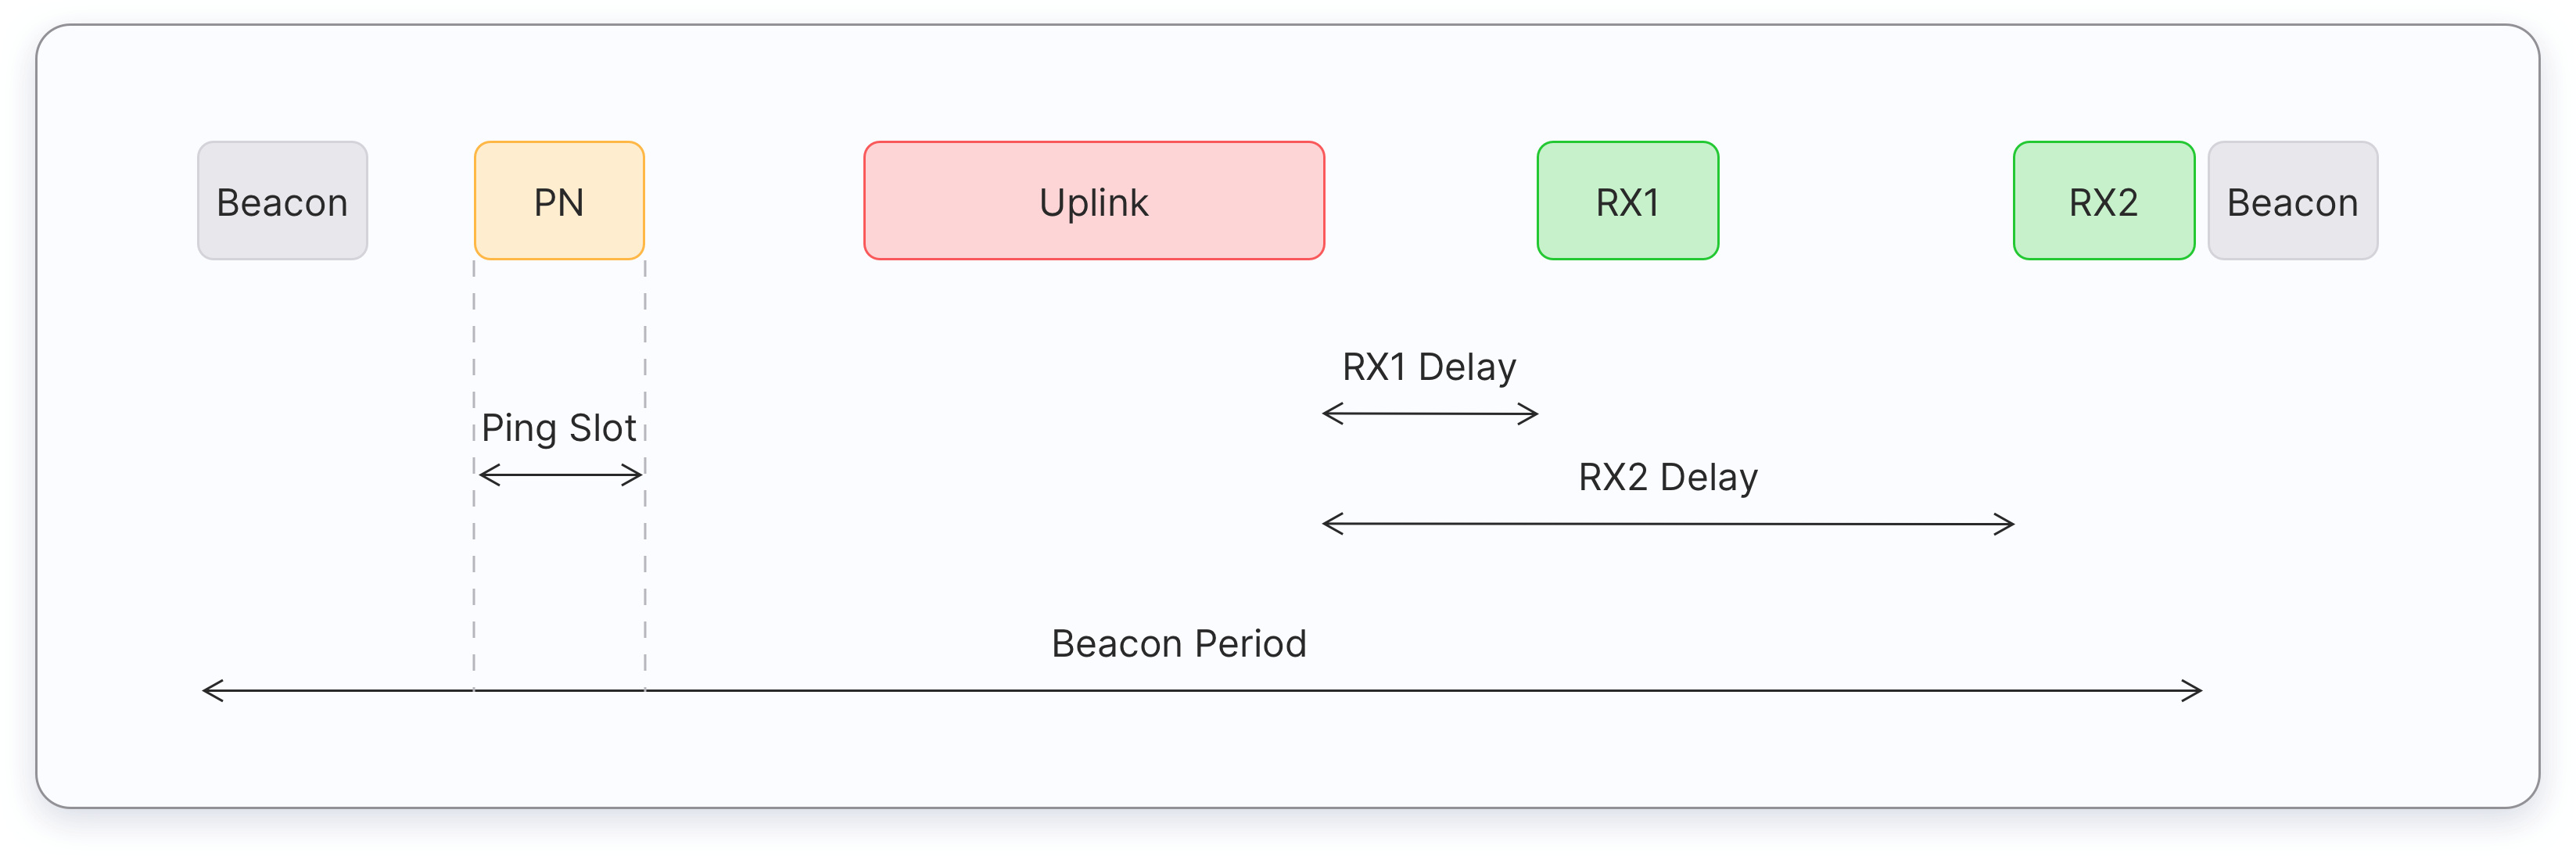
\includegraphics[width=0.8\textwidth]{figures/class-b.png}
    \caption{LoRaWAN Class B Operation}
    \label{fig:lora_class_b}
\end{figure}
Class B extends Class A by introducing scheduled receive slots—known as \emph{ping slots}—to reduce downlink latency while maintaining reasonable power efficiency.
Figure~\ref{fig:lora_class_b} illustrates the timing of uplink and downlink transmissions in Class B devices.
\begin{enumerate}
    \item Gateways periodically broadcast synchronized \emph{beacons} (every 128 seconds by default), which provide a common time reference.
    \item End-devices use these beacons to align their internal clocks with network time.
    \item Based on this synchronization, the Network Server can schedule downlinks during predefined ping slots assigned to individual devices or multicast groups.
    \item After each uplink, the device still opens RX1 and RX2 windows as in Class A.
    \item Ping slots occur at regular intervals determined by \texttt{PING\_SLOT\_PERIODICITY} (default: $2^7 = 128$ seconds).
\end{enumerate}

Class B offers medium downlink latency and is suitable for applications requiring occasional actuation or more frequent downlink interaction than Class A permits. Power consumption is higher than Class A due to periodic beacon reception and ping slot listening, but many Class B devices remain battery-operated with acceptable lifespans.

Typical use cases include:

\begin{enumerate}
    \item Utility meters (electricity, water, gas)
    \item Smart street lighting systems
\end{enumerate}

Class B devices may revert to Class A operation when ping slot functionality is not required.

\subsection{Class C}
\begin{figure}
    \centering
    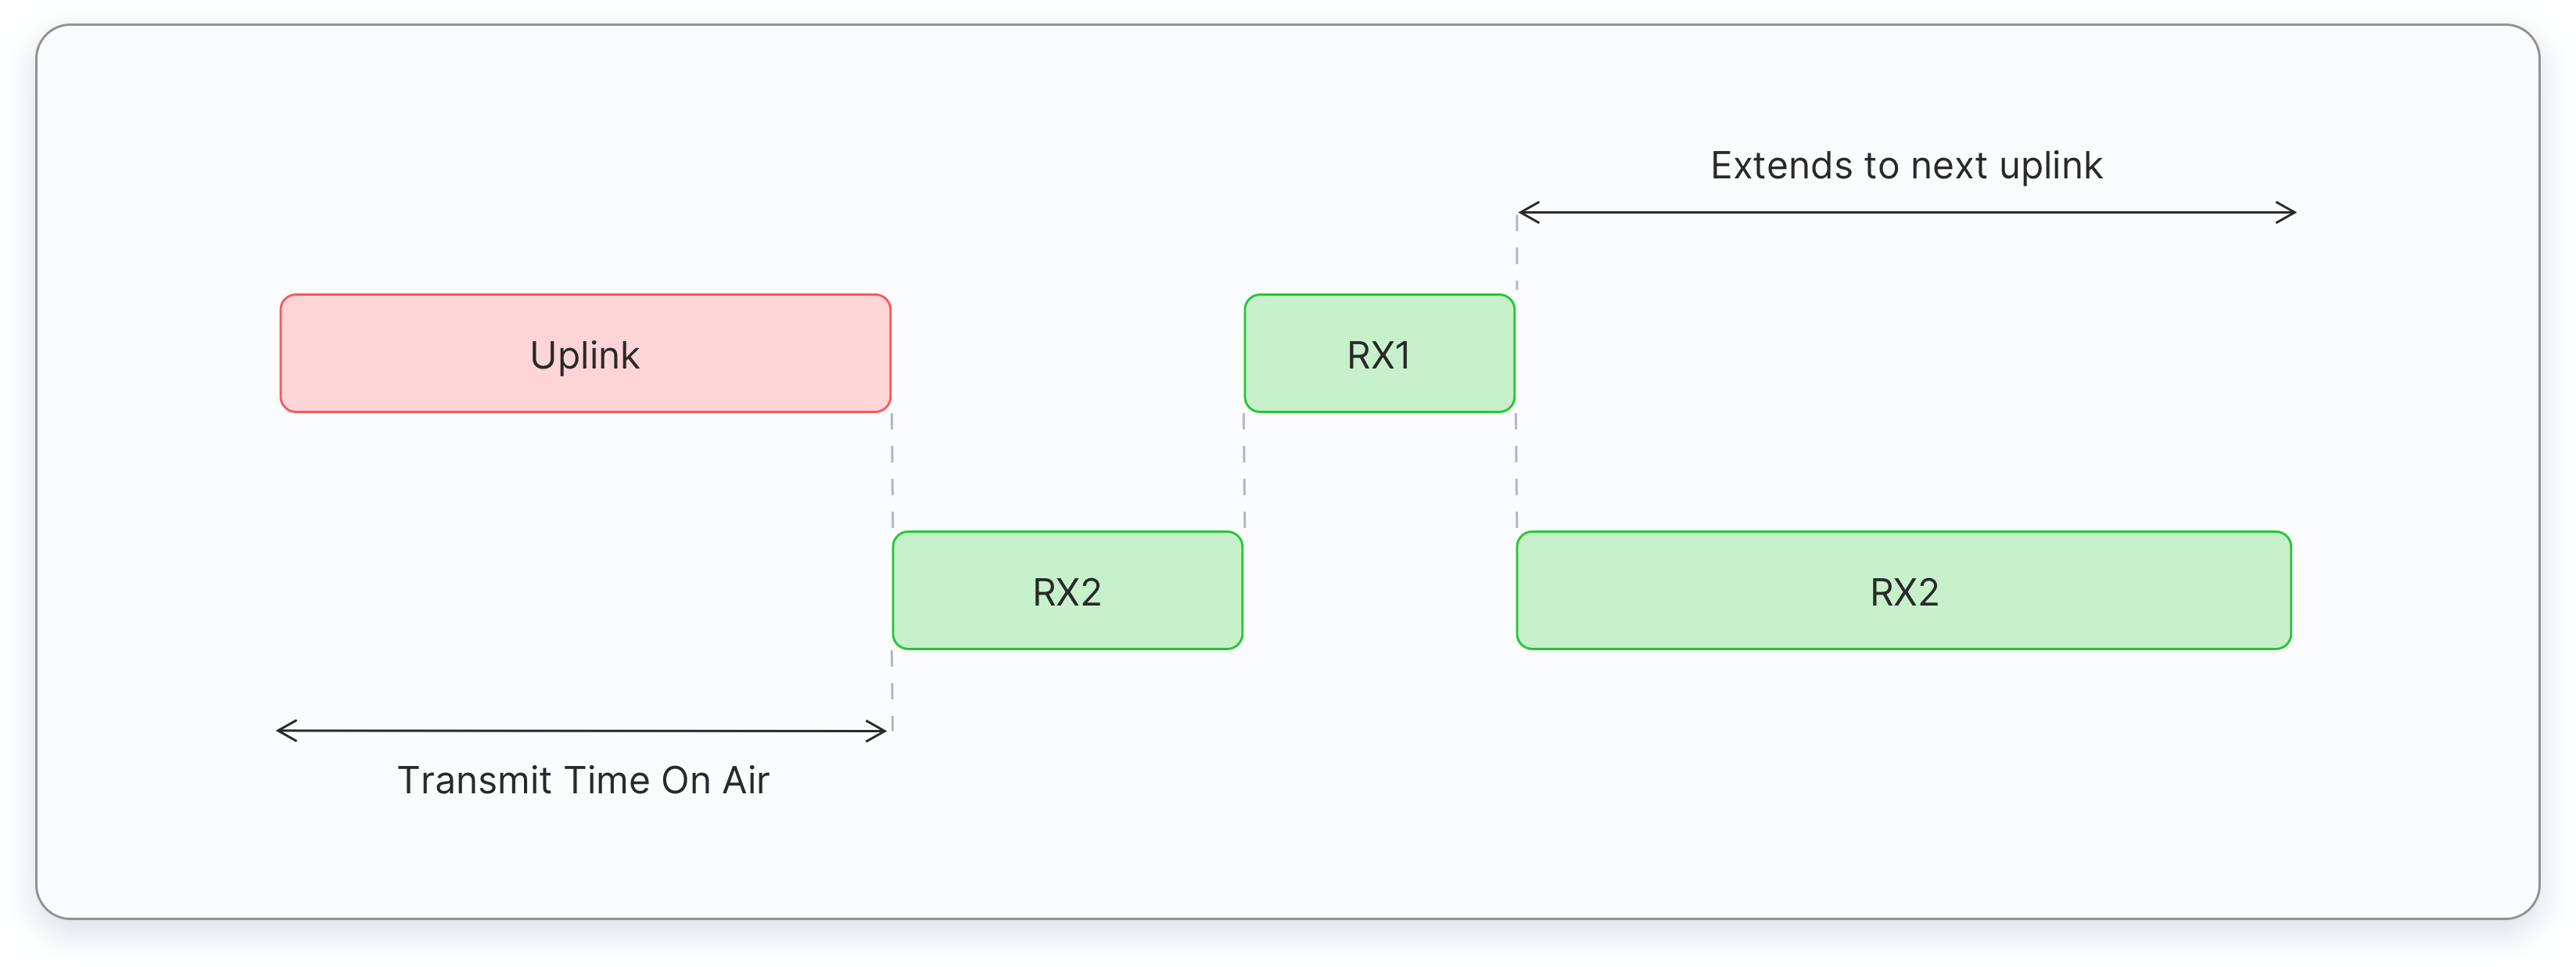
\includegraphics[width=0.8\textwidth]{figures/class-c.png}
    \caption{LoRaWAN Class C Operation}
    \label{fig:lora_class_c}
\end{figure}
Class C provides the lowest possible downlink latency by keeping the receiver nearly always active, at the expense of significantly higher power consumption.
Figure~\ref{fig:lora_class_c} illustrates the timing of uplink and downlink transmissions in Class C devices.

\begin{enumerate}
    \item After an uplink transmission, the device opens RX1 and RX2 as in Class A.
    \item Following RX2, the device keeps the RX2 receive window \emph{continuously open} until the next uplink transmission is initiated.
    \item This allows the Network Server to send downlink messages at any time, subject only to regulatory duty cycle constraints.
    \item Uplink transmissions are only possible when no downlink is in progress.
\end{enumerate}

Due to the near-continuous radio activity, Class C devices are generally unsuitable for long-term battery operation and are typically mains-powered.

Common applications include:

\begin{enumerate}
    \item Utility meters requiring real-time control
    \item Street lights with dynamic dimming or on/off commands
    \item Beacon lights and alarm systems requiring immediate response
\end{enumerate}

Class C devices may operate in Class A mode during low-activity periods to conserve energy, though this requires explicit mode switching via MAC commands or application logic.


\section{End Device Activation}

Prior to participating in a LoRaWAN network, every end device must undergo an activation procedure to establish cryptographic credentials and obtain a network address. Two distinct activation methods are defined in the LoRaWAN specification: Over-the-Air Activation (OTAA) and Activation by Personalization (ABP). OTAA is the recommended and more secure approach, enabling dynamic key derivation and network roaming, whereas ABP involves pre-provisioning of static keys and addresses, limiting flexibility and security.

\subsection{Over-the-Air Activation in LoRaWAN 1.0.x}
\begin{figure}[htbp]
    \centering
    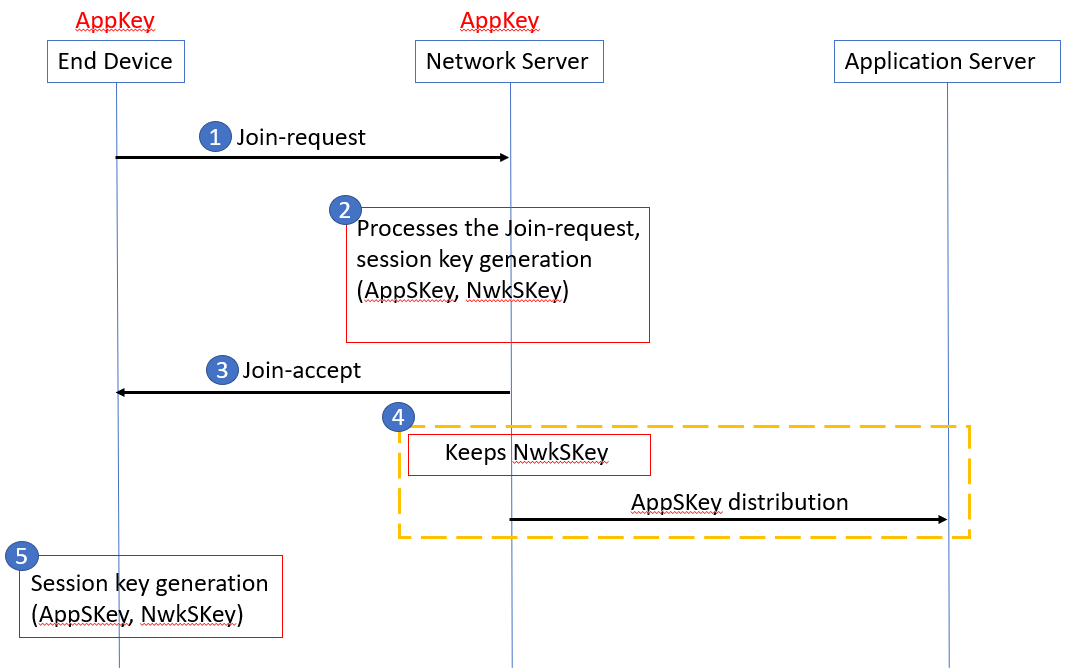
\includegraphics[width=0.8\textwidth]{figures/otaa-lorawan1.0.png}
    \caption{LoRaWAN 1.0.x Over-the-Air Activation (OTAA) Procedure}
    \label{fig:lora_otaa_1.0}
\end{figure}

In LoRaWAN 1.0.x, OTAA is accomplished through a two-message handshake between the end device and the Network Server, facilitated by a shared root key. The procedure is as follows:
Figure~\ref{fig:lora_otaa_1.0} illustrates the OTAA process in LoRaWAN 1.0.x.

\begin{enumerate}
    \item \textbf{Prerequisites}: The end device must be provisioned with the following non-volatile parameters:
          \begin{enumerate}
              \item \texttt{AppEUI}: A 64-bit IEEE EUI-64 identifier of the application server.
              \item \texttt{DevEUI}: A 64-bit IEEE EUI-64 unique identifier of the end device.
              \item \texttt{AppKey}: A 128-bit AES secret root key, shared with the Network Server.
          \end{enumerate}
          The \texttt{AppKey} is never transmitted over the air.

    \item \textbf{Join-request transmission}: The end device initiates the join procedure by transmitting a \texttt{Join-request} message containing:
          \begin{enumerate}
              \item \texttt{AppEUI} (8 bytes)
              \item \texttt{DevEUI} (8 bytes)
              \item \texttt{DevNonce} (2 bytes): a random or monotonically increasing nonce to prevent replay attacks.
          \end{enumerate}
          The Message Integrity Code (MIC) is computed over these fields using \texttt{AppKey} in AES-CMAC. The message is sent unencrypted on one of the region-specific join channels (e.g., 868.10/868.30/868.50 MHz in EU868).

    \item \textbf{Join-accept generation}: Upon successful validation, the Network Server generates:
          \begin{enumerate}
              \item A 32-bit dynamic \texttt{DevAddr}.
              \item Two 128-bit session keys: \texttt{NwkSKey} (for network-layer integrity and MAC command encryption) and \texttt{AppSKey} (for application payload encryption).
              \item A \texttt{Join-accept} message comprising:
              \item \texttt{AppNonce} (3 bytes): server-provided nonce.
              \item \texttt{NetID} (3 bytes): network identifier.
              \item \texttt{DevAddr} (4 bytes)
              \item \texttt{DLSettings} (1 byte): downlink configuration.
              \item \texttt{RxDelay} (1 byte): receive window delay.
              \item \texttt{CFList} (0 or 16 bytes, optional): additional channel frequencies.
          \end{enumerate}
          The MIC of the \texttt{Join-accept} is computed using \texttt{AppKey}, and the entire payload is encrypted with \texttt{AppKey} using AES-128 in ECB mode.

    \item \textbf{Join-accept delivery}: The encrypted \texttt{Join-accept} is delivered to the end device via a downlink in RX1 or RX2. No response is sent if the request is rejected.

    \item \textbf{Session key derivation and activation}: The end device decrypts the \texttt{Join-accept} and derives \texttt{NwkSKey} and \texttt{AppSKey} using \texttt{AppKey} and \texttt{AppNonce}. The device stores:
          \begin{enumerate}
              \item \texttt{DevAddr}
              \item \texttt{NwkSKey}
              \item \texttt{AppSKey}
          \end{enumerate}
          The Network Server retains \texttt{NwkSKey}, while \texttt{AppSKey} is forwarded to the Application Server.
\end{enumerate}

\subsection{Over-the-Air Activation in LoRaWAN 1.1}
\begin{figure}[htbp]
    \centering
    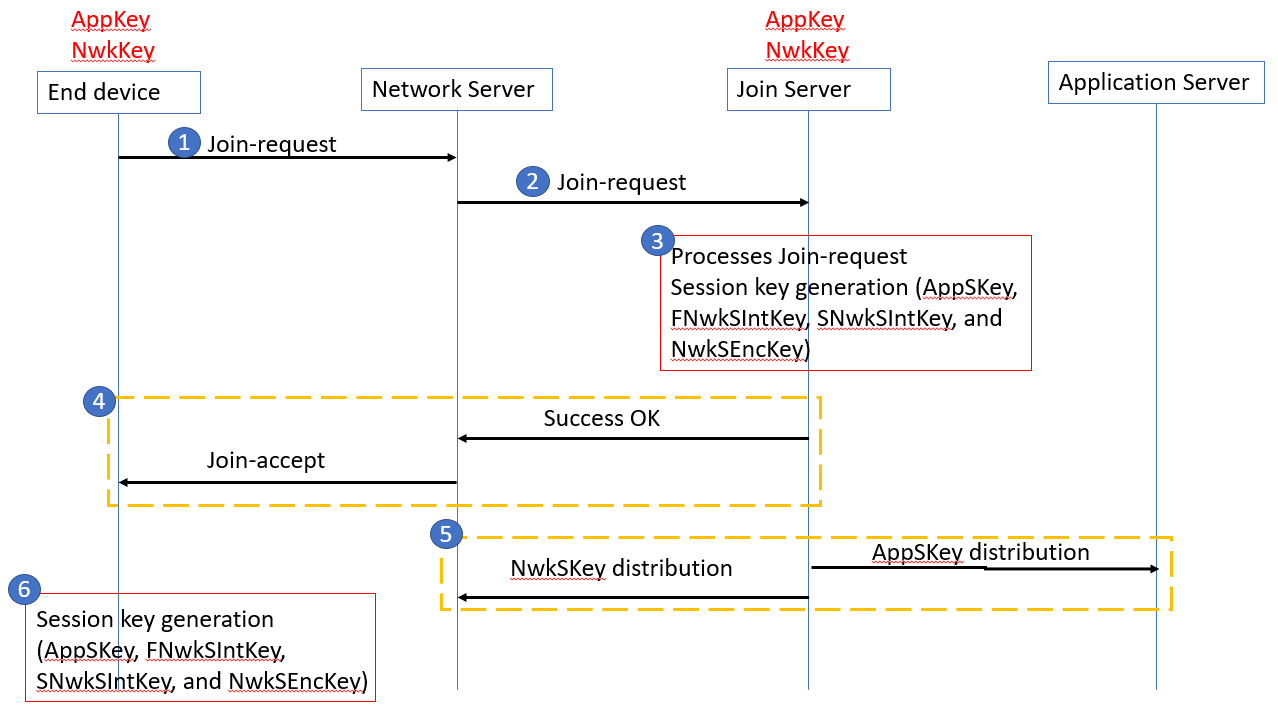
\includegraphics[width=0.8\textwidth]{figures/otaa-1.1.png}
    \caption{LoRaWAN 1.1 Over-the-Air Activation (OTAA) Procedure}
    \label{fig:lora_otaa_1.1}
\end{figure}
LoRaWAN 1.1 enhances security by separating network and application root keys and introducing a dedicated Join Server. The OTAA procedure involves the following steps:
Figure~\ref{fig:lora_otaa_1.1} illustrates the OTAA process in LoRaWAN 1.1.

\begin{enumerate}
    \item \textbf{Prerequisites}: The end device is provisioned with:
          \begin{enumerate}
              \item \texttt{JoinEUI}: 64-bit identifier of the Join Server (replaces \texttt{AppEUI}).
              \item \texttt{DevEUI}: 64-bit device identifier.
              \item \texttt{AppKey}: root key for application session derivation.
              \item \texttt{NwkKey}: root key for network session derivation.
          \end{enumerate}
          Both \texttt{AppKey} and \texttt{NwkKey} are kept secret and never transmitted.

    \item \textbf{Join-request transmission}: The end device sends a \texttt{Join-request} containing:
          \begin{enumerate}
              \item \texttt{JoinEUI} (8 bytes)
              \item \texttt{DevEUI} (8 bytes)
              \item \texttt{DevNonce} (2 bytes): typically a counter incremented per join attempt.
          \end{enumerate}
          The MIC is computed using \texttt{NwkKey}. The message is unencrypted and transmitted on region-specific join channels.

    \item \textbf{Forwarding to Join Server}: The Network Server forwards the validated \texttt{Join-request} to the Join Server identified by \texttt{JoinEUI}.

    \item \textbf{Session key generation}: The Join Server derives four session keys:
          \begin{enumerate}
              \item \texttt{AppSKey}: for application payload confidentiality.
              \item \texttt{FNwkSIntKey}: for uplink MIC (first part).
              \item \texttt{SNwkSIntKey}: for uplink MIC (second part) and all downlink MICs.
              \item \texttt{NwkSEncKey}: for MAC command encryption in both directions.
          \end{enumerate}

    \item \textbf{Join-accept construction and encryption}: The Network Server constructs the \texttt{Join-accept} message with:
          \begin{enumerate}
              \item \texttt{JoinNonce} (1 byte): Join Server-provided nonce.
              \item \texttt{NetID} (3 bytes)
              \item \texttt{DevAddr} (4 bytes)
              \item \texttt{DLSettings} (1 byte)
              \item \texttt{RxDelay} (1 byte)
              \item \texttt{CFList} (0 or 16 bytes, optional)
          \end{enumerate}
          The MIC is computed using \texttt{JSIntKey} (derived from \texttt{NwkKey}), and the payload is encrypted with \texttt{NwkKey} (for \texttt{Join-request}) or \texttt{JSEncKey} (for \texttt{Rejoin-request}).

    \item \textbf{Key distribution}: The Join Server sends \texttt{AppSKey} to the Application Server and the three network keys (\texttt{FNwkSIntKey}, \texttt{SNwkSIntKey}, \texttt{NwkSEncKey}) to the Network Server.

    \item \textbf{Device activation}: The end device decrypts the \texttt{Join-accept} and derives all four session keys using \texttt{AppKey}, \texttt{NwkKey}, and \texttt{JoinNonce}. It stores:
          \begin{enumerate}
              \item \texttt{DevAddr}
              \item \texttt{AppSKey}
              \item \texttt{FNwkSIntKey}
              \item \texttt{SNwkSIntKey}
              \item \texttt{NwkSEncKey}
          \end{enumerate}
\end{enumerate}

\subsection{Activation by Personalization}
\begin{figure}
    \centering
    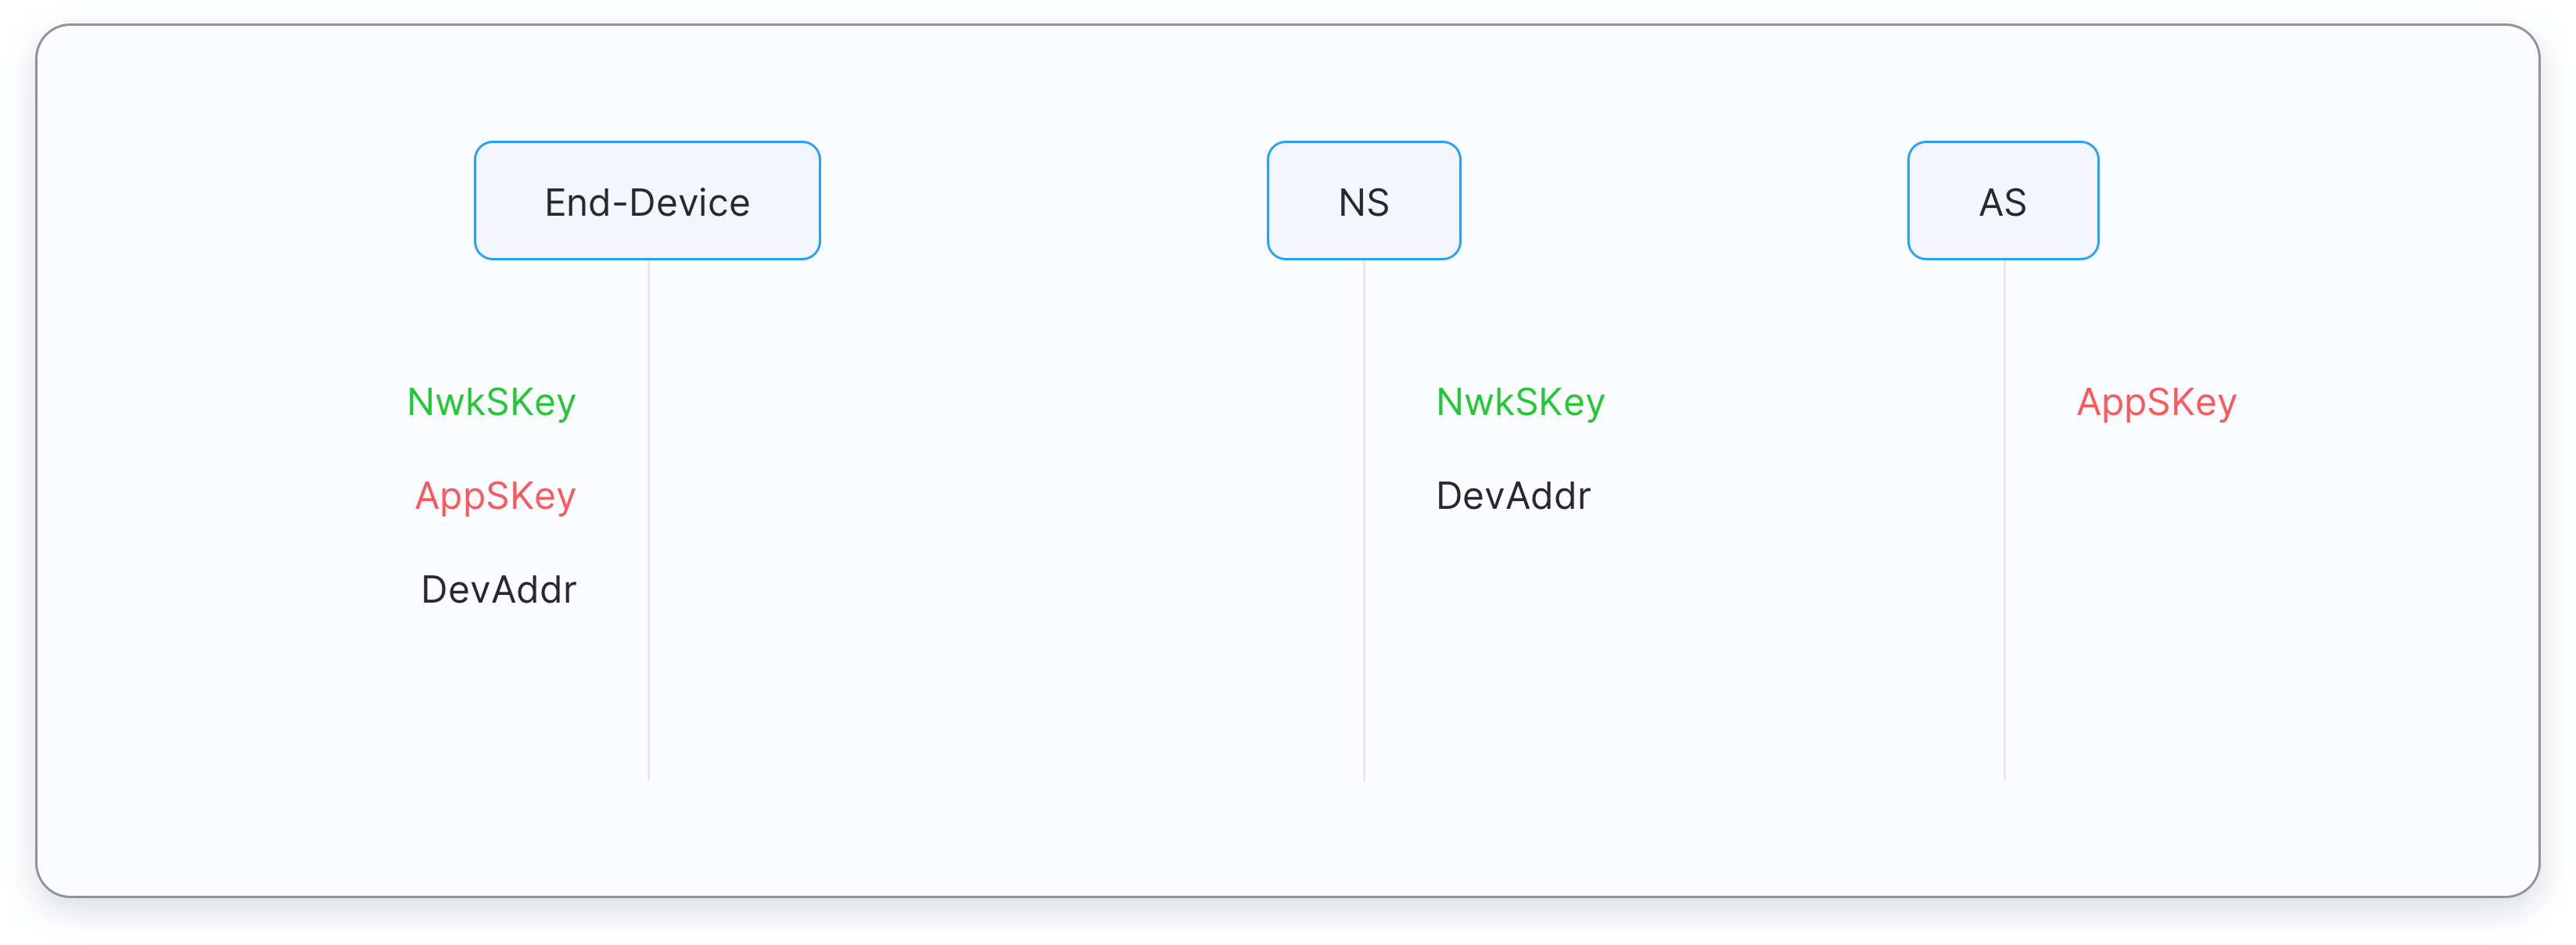
\includegraphics[width=0.8\textwidth]{figures/abp-1.0.png}
    \caption{LoRaWAN Activation by Personalization (ABP) Procedure}
    \label{fig:lora_abp}
\end{figure}

Activation by Personalization (ABP) bypasses the join procedure by pre-configuring session parameters directly into the end device. This method is less secure and does not support network roaming.
Figure~\ref{fig:lora_abp} illustrates the ABP process.

\begin{figure}
    \centering
    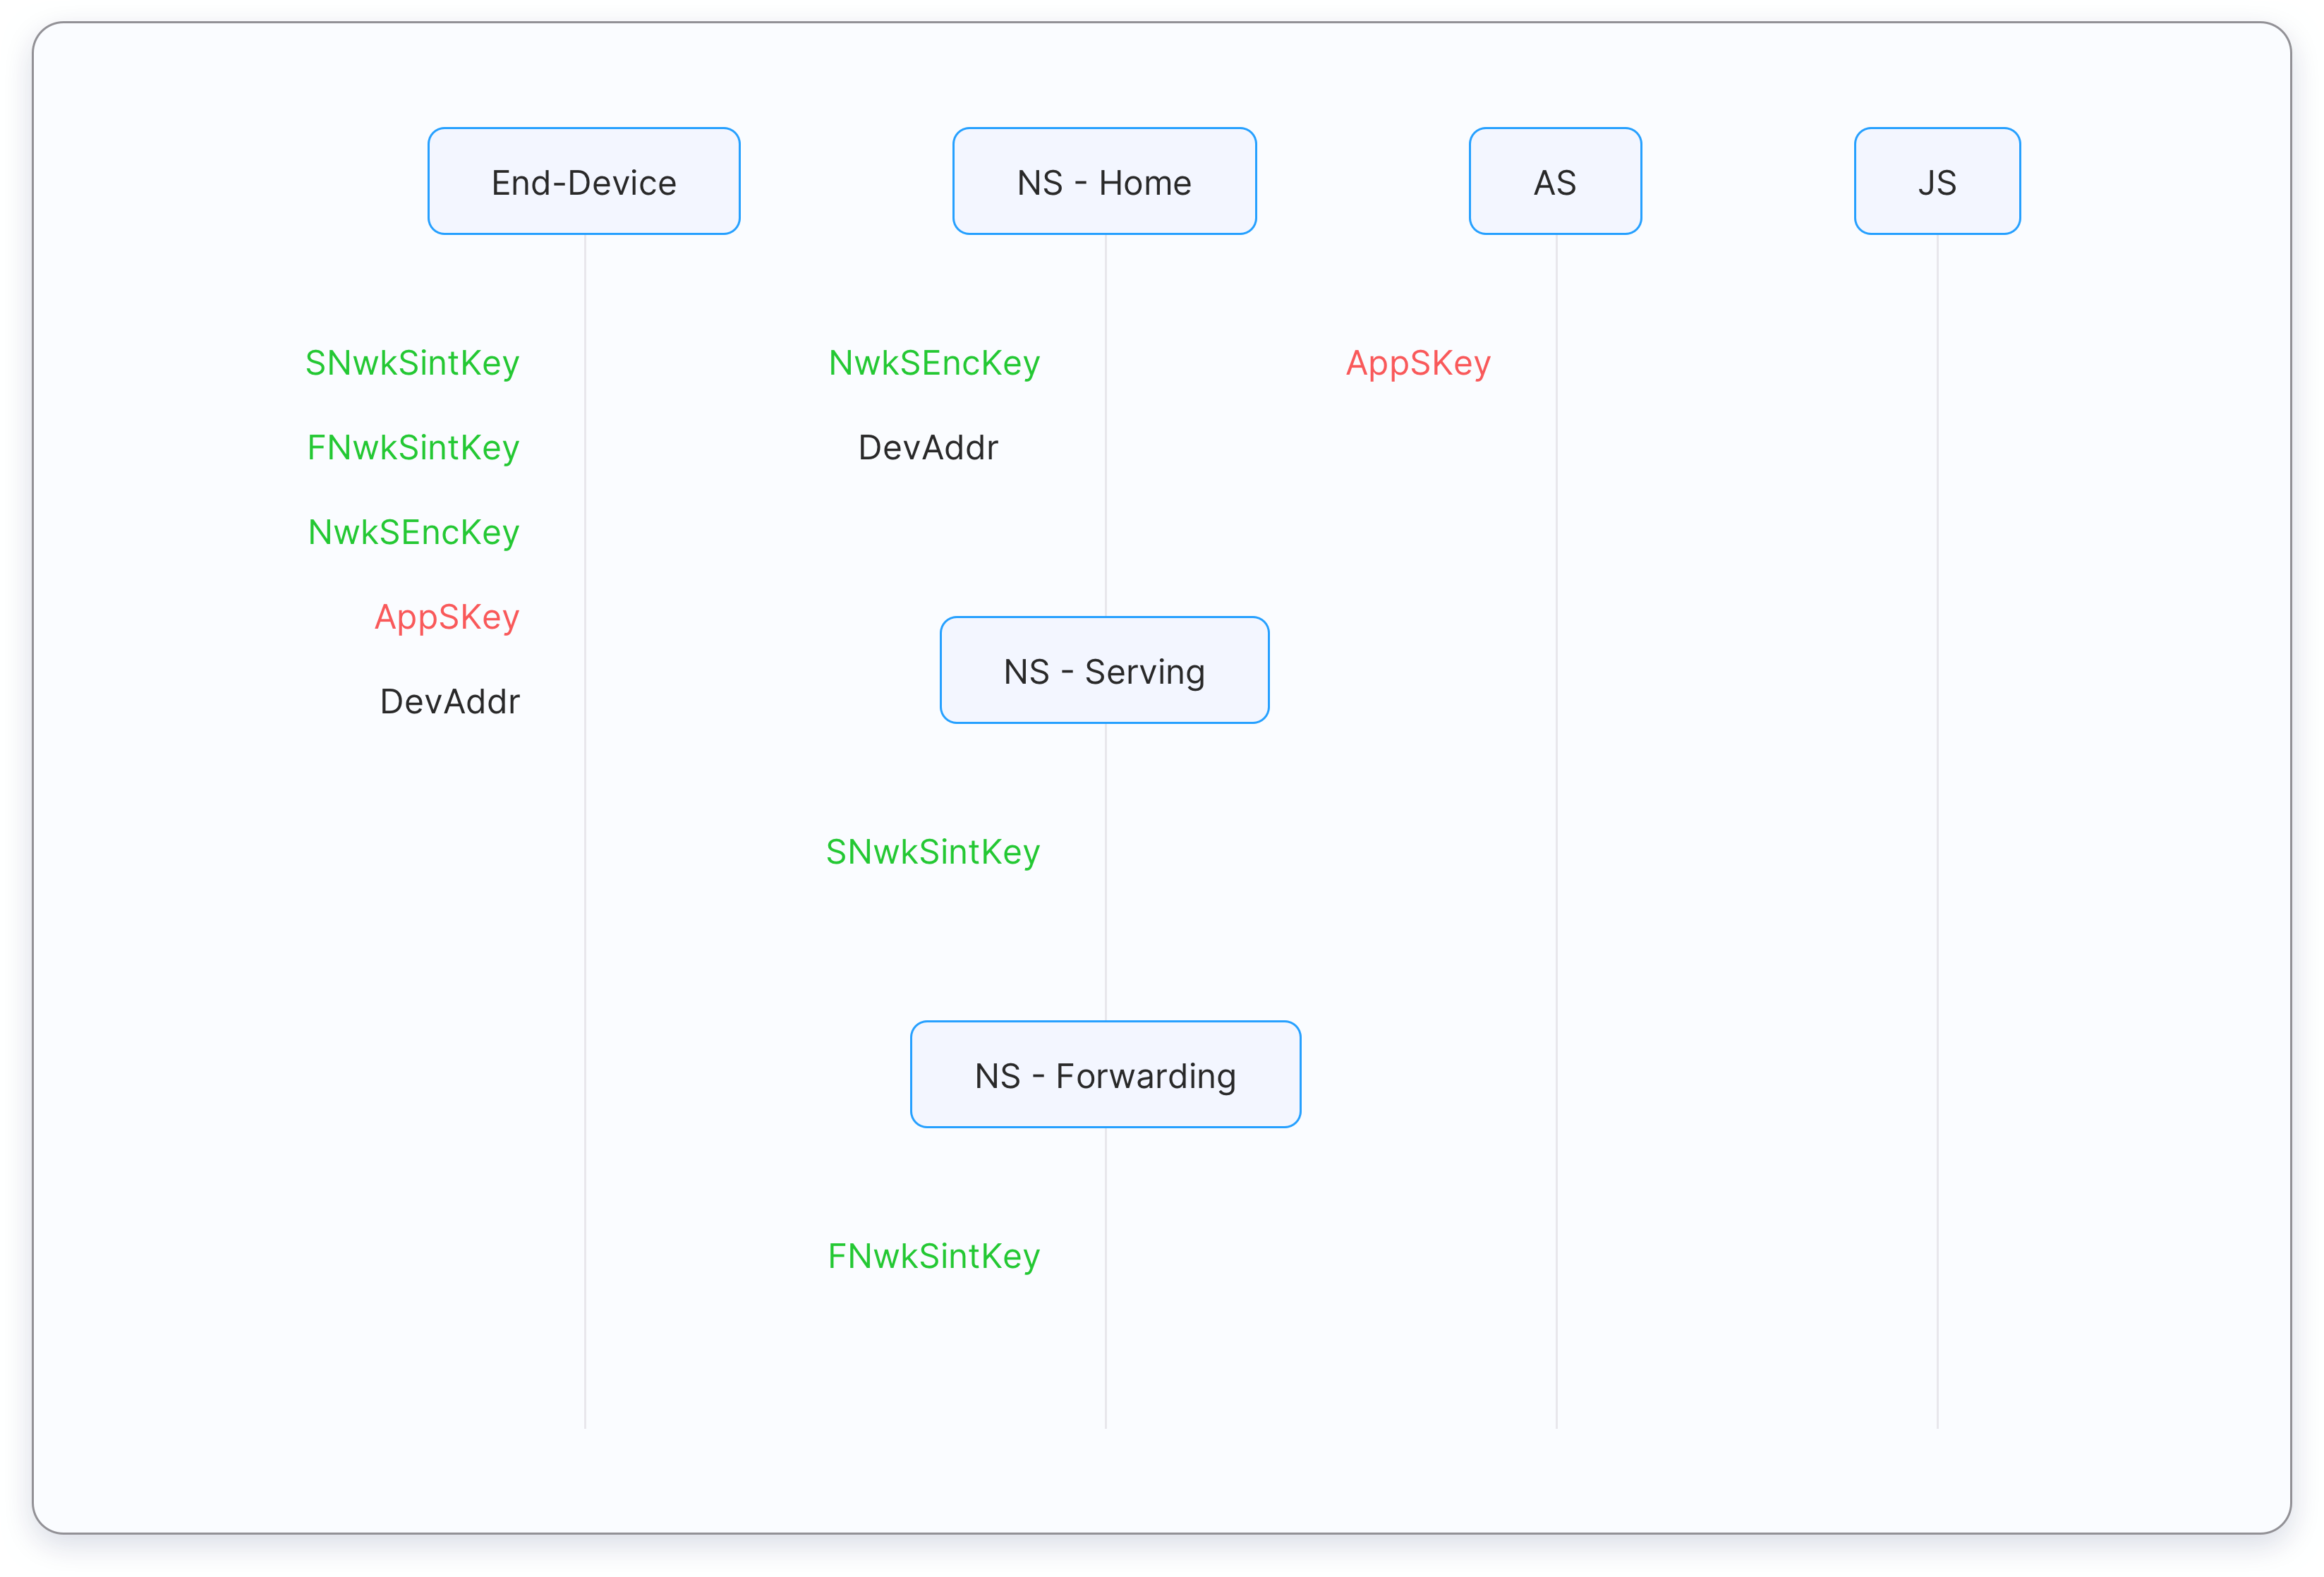
\includegraphics[width=0.8\textwidth]{figures/abp-1.1.png}
    \caption{LoRaWAN 1.1 Activation by Personalization (ABP) Procedure}
    \label{fig:lora_abp_1.1}
\end{figure}
In LoRaWAN 1.1, ABP requires pre-provisioning of multiple session keys to align with the enhanced security model.
Figure~\ref{fig:lora_abp_1.1} illustrates the ABP process in LoRaWAN 1.1.

\begin{enumerate}
    \item \textbf{ABP in LoRaWAN 1.0.x}: The following parameters are pre-provisioned:
          \begin{enumerate}
              \item \texttt{DevAddr} (32 bits)
              \item \texttt{NwkSKey} (128 bits)
              \item \texttt{AppSKey} (128 bits)
          \end{enumerate}
          These must be manually synchronized with the Network Server (\texttt{DevAddr}, \texttt{NwkSKey}) and Application Server (\texttt{AppSKey}).

    \item \textbf{ABP in LoRaWAN 1.1}: Four session keys are pre-provisioned:
          \begin{enumerate}
              \item \texttt{DevAddr} (32 bits)
              \item \texttt{FNwkSIntKey} (128 bits)
              \item \texttt{SNwkSIntKey} (128 bits)
              \item \texttt{NwkSEncKey} (128 bits)
              \item \texttt{AppSKey} (128 bits)
          \end{enumerate}
          The Network Server stores the three network keys and \texttt{DevAddr}, while the Application Server stores \texttt{AppSKey}.

    \item \textbf{Security implications}: ABP devices use static session keys for their entire lifetime, increasing vulnerability to key compromise. Additionally, changing network providers requires manual reconfiguration of all cryptographic material.
\end{enumerate}



\section{Spreading Factors}

LoRa employs Chirp Spread Spectrum (CSS) modulation, wherein information is encoded in linear frequency-modulated pulses known as \emph{chirps} or \emph{symbols}. The \emph{spreading factor} (SF) is a fundamental parameter that governs the duration and structure of each chirp, thereby directly influencing key transmission characteristics including data rate, communication range, time-on-air, receiver sensitivity, and energy consumption.

\subsection{Definition and Impact of Spreading Factor}

\begin{enumerate}
    \item The spreading factor determines the chirp sweep rate: a higher spreading factor corresponds to a slower chirp, which increases the symbol duration and reduces the data rate.
    \item For each unit increment in spreading factor (e.g., from SF7 to SF8), the chirp duration doubles, and consequently the data rate is halved for a fixed bandwidth and coding rate.
    \item LoRa supports six spreading factors, denoted SF7 through SF12, where SF7 yields the highest data rate and shortest range, while SF12 provides the lowest data rate and longest range.
    \item Spreading factors are orthogonal: transmissions using different spreading factors on the same frequency and at the same time do not interfere, enabling spectral reuse and congestion management in dense networks.
\end{enumerate}

\subsection{Data Rate}

\begin{enumerate}
    \item For a fixed bandwidth and coding rate, the data rate is inversely proportional to the spreading factor.
    \item The data rate is directly proportional to the bandwidth: doubling the bandwidth doubles the data rate for a given spreading factor.
    \item Example bit rates for SF7 with coding rate 4/5 (often simplified as CR = 1 in nominal calculations) are:
          \begin{enumerate}
              \item 5.5 kbit/s at 125 kHz bandwidth
              \item 10.9 kbit/s at 250 kHz bandwidth
              \item 21.9 kbit/s at 500 kHz bandwidth
          \end{enumerate}
\end{enumerate}

\subsection{Communication Range}

\begin{enumerate}
    \item Higher spreading factors increase the processing gain, enhancing the signal’s resilience to noise and enabling reception at lower signal-to-noise ratios (SNR).
    \item As a result, transmissions using SF12 achieve significantly greater range than those using SF7 under identical power and environmental conditions.
    \item This property allows the network to dynamically adjust the spreading factor per device to balance data rate and coverage based on link quality.
\end{enumerate}

\subsection{Time-on-Air}

\begin{enumerate}
    \item Time-on-air refers to the duration a device occupies the channel to transmit a given payload.
    \item For a fixed payload size and bandwidth, time-on-air increases exponentially with the spreading factor.
    \item Longer time-on-air may exacerbate duty cycle limitations in regulated bands and increase vulnerability to interference.
    \item Network operators often use airtime calculators (e.g., The Things Network’s LoRaWAN airtime calculator) to estimate transmission duration based on payload size, bandwidth, and spreading factor.
\end{enumerate}

\subsection{Receiver Sensitivity}

\begin{enumerate}
    \item Receiver sensitivity—the minimum signal power at which a receiver can correctly decode a transmission—improves with higher spreading factors.
    \item For a fixed bandwidth of 125 kHz, typical receiver sensitivity values are:
          \begin{enumerate}
              \item SF7: \SI{-123}{\decibel m}
              \item SF8: \SI{-126}{\decibel m}
              \item SF9: \SI{-129}{\decibel m}
              \item SF10: \SI{-132}{\decibel m}
              \item SF11: \SI{-134.5}{\decibel m}
              \item SF12: \SI{-137}{\decibel m}
          \end{enumerate}
    \item This enhanced sensitivity at high spreading factors is critical for maintaining connectivity in low-signal environments, such as deep indoor or rural deployments.
\end{enumerate}

\subsection{Battery Life}

\begin{enumerate}
    \item Radio transmission is the dominant source of energy consumption in LoRaWAN end devices.
    \item Higher spreading factors increase the time-on-air, which directly increases the active transmission time and thus energy expenditure per message.
    \item Consequently, devices operating predominantly at SF12 will exhibit shorter battery life compared to those operating at SF7, assuming identical payload sizes and transmission frequencies.
    \item Adaptive Data Rate (ADR) mechanisms in LoRaWAN aim to minimize spreading factor (and thus power consumption) while maintaining link reliability, thereby optimizing battery longevity.
\end{enumerate}

\section{Adaptive Data Rate}

Adaptive Data Rate (ADR) is a network-controlled mechanism designed to optimize the trade-off between communication reliability, airtime utilization, and energy consumption in LoRaWAN networks. By dynamically adjusting transmission parameters based on observed link quality, ADR enables efficient spectrum usage while maintaining robust connectivity.

\subsection{Transmission Parameters Controlled by ADR}

The ADR mechanism governs the following physical layer parameters of an end device:

\begin{enumerate}
    \item Spreading factor
    \item Bandwidth
    \item Transmission power
\end{enumerate}

Devices in close proximity to gateways typically operate with a lower spreading factor and higher data rate to minimize airtime and energy expenditure. Conversely, devices at the cell edge utilize higher spreading factors to achieve the necessary link budget for reliable reception.

\subsection{Conditions for ADR Activation}

ADR should be enabled only under stable radio frequency (RF) conditions. Consequently:

\begin{enumerate}
    \item Static end devices may generally enable ADR, provided the RF environment remains consistent.
    \item If a static device detects temporary RF degradation (e.g., due to environmental obstruction such as a vehicle parked over a sensor), it should temporarily disable ADR.
    \item Mobile end devices should implement logic to detect periods of prolonged stationary operation and enable ADR during such intervals.
    \item The decision to enable or disable ADR resides exclusively with the end device; neither the application server nor the network server may override this decision.
\end{enumerate}

\subsection{ADR Operation in The Things Stack}

The Things Stack implements ADR using a measurement-based optimization algorithm derived from Semtech’s recommended rate adaptation strategy. Key operational aspects include:

\begin{enumerate}
    \item Upon setting the ADR bit in an uplink frame, the Network Server begins collecting the most recent 20 uplink measurements. Each measurement includes:
          \begin{enumerate}
              \item Frame counter
              \item Signal-to-Noise Ratio (SNR) reported by the best-receiving gateway
              \item Number of gateways that received the message
          \end{enumerate}

    \item When the ADR bit is cleared by the device (e.g., due to mobility or unstable RF conditions), all prior measurements are discarded. Measurement collection resumes only after the ADR bit is reasserted.

    \item For each measurement, a \emph{margin} is computed as:
          \[
              \text{Margin} = \text{Measured SNR} - \text{Required SNR for current data rate}
          \]
          This margin quantifies the excess link budget, which informs potential increases in data rate or reductions in transmit power.

    \item ADR requests are triggered under the following conditions:
          \begin{enumerate}
              \item \textbf{Initial ADR Request (US915 and AU915 only)}: Sent immediately after join in pre-LoRaWAN 1.1 deployments to configure the channel mask. This request incorporates a safety margin due to insufficient link measurements at join time. LoRaWAN 1.1 eliminates the need for this request by allowing channel mask configuration in the \texttt{JoinAccept} message.
              \item \textbf{Regular ADR Request}: Scheduled when sufficient measurements indicate suboptimal data rate or power settings. The request is piggybacked on an existing application-layer downlink (e.g., an ACK or payload).
              \item \textbf{Lowest Data Rate Trigger}: Sent when the device operates at DR0 (typically SF12/125 kHz), regardless of margin, to encourage rate adaptation.
              \item \textbf{ADR Acknowledgment Request}: Triggered when the device sets the \texttt{ADRAckReq} bit, typically after transmitting 64 uplinks without receiving a downlink (implementation-dependent).
          \end{enumerate}

    \item If an end device repeatedly rejects ADR commands, the Network Server ceases scheduling further ADR requests. This behavior may indicate either a device firmware issue or a version incompatibility between the device and server.
\end{enumerate}

\section{Limitations and Design Recommendations}

LoRaWAN is a specialized Low Power Wide Area Network (LPWAN) protocol optimized for specific classes of Internet of Things (IoT) applications. While it offers significant advantages in terms of range, energy efficiency, and cost, it is inherently unsuited for use cases requiring high data rates, low latency, or continuous communication. Understanding these limitations is essential for effective system design and resource utilization.

\subsection{Appropriate Use Cases for LoRaWAN}

LoRaWAN is well-suited for applications exhibiting the following characteristics:

\begin{enumerate}
    \item \textbf{Long-range communication}: Capable of achieving coverage over multiple kilometers in rural environments and several hundred meters to a few kilometers in urban settings.
    \item \textbf{Ultra-low power consumption}: End-devices can operate for several years on a single battery due to duty-cycled operation and efficient sleep modes.
    \item \textbf{Low capital and operational expenditure}: Hardware costs are typically below 20\,\texteuro\ per node, with minimal recurring operational expenses.
    \item \textbf{Low data rate requirements}: Physical layer bit rates range from approximately 250\,bit/s to 11\,kbit/s in the EU868 band (using LoRa modulation), depending on the selected spreading factor and bandwidth.
    \item \textbf{Decentralized network deployment}: Users may deploy private gateways to achieve coverage in remote or underserved areas without reliance on third-party infrastructure.
    \item \textbf{End-to-end security}: All application payloads are encrypted using 128-bit AES, ensuring confidentiality and integrity.
\end{enumerate}

\subsection{Inappropriate Use Cases for LoRaWAN}

LoRaWAN is not designed for the following scenarios:

\begin{enumerate}
    \item \textbf{Real-time or high-frequency data transmission}: The protocol enforces regulatory duty cycles and is optimized for infrequent transmissions (e.g., once every few minutes).
    \item \textbf{Voice or audio communication}: Technologies such as GPRS, 3G, or LTE are more appropriate for voice-grade services.
    \item \textbf{Short-range, high-interaction control systems}: Protocols like Zigbee or Bluetooth Low Energy (BLE) are better suited for in-home automation (e.g., lighting control).
    \item \textbf{High-bandwidth applications}: Transmission of images, video streaming (e.g., Netflix), or large files is infeasible; Wi-Fi or cellular broadband should be used instead.
\end{enumerate}

\subsection{Uplink Transmission Best Practices}

To maximize spectral efficiency, battery life, and network capacity, the following guidelines should be observed for uplink communications:

\begin{enumerate}
    \item \textbf{Minimize payload size}: Data should be encoded in compact binary formats rather than verbose representations such as JSON or ASCII text. The Cayenne Low Power Payload (LPP) format is recommended for its simplicity and widespread support.
    \item \textbf{Optimize transmission frequency}: Messages should be transmitted at intervals of several minutes. Data aggregation strategies—such as reporting minimum, average, and maximum values over a window—or event-driven transmission (e.g., triggered by threshold crossing or motion detection) can significantly reduce unnecessary traffic.
    \item \textbf{Use the highest feasible data rate}: A higher data rate (e.g., SF7 with 125\,kHz bandwidth) minimizes time-on-air and energy consumption. If link margin is insufficient, the spreading factor may be incrementally increased. Adaptive Data Rate (ADR) should be enabled where RF conditions are stable, allowing the network server to dynamically optimize the data rate and transmit power.
\end{enumerate}

\subsection{Downlink Transmission Best Practices}

Due to the half-duplex nature of most LoRaWAN gateways, downlink transmissions temporarily disable the gateway’s ability to receive uplink messages across all channels. This impacts network capacity and reliability. Therefore, the following constraints apply:

\begin{enumerate}
    \item \textbf{Minimize downlink usage}: Downlink messages should be avoided unless absolutely necessary for application functionality.
    \item \textbf{Keep downlink payloads small}: When downlinks are required, payload size should be minimized to reduce airtime.
    \item \textbf{Optimize uplink to improve downlink efficiency}: The downlink data rate is derived from the uplink data rate and RX1DROffset. Efficient uplink configurations (e.g., high data rates) enable correspondingly efficient downlinks.
    \item \textbf{Avoid confirmed uplinks unless essential}: Confirmed uplink messages trigger mandatory downlink acknowledgments, increasing network load. Applications should be designed to tolerate occasional message loss where possible, using application-layer reliability mechanisms if needed.
\end{enumerate}




% \section{Campus Based IoT Test Bed}
% The Campus Based IoT Test Bed (C-IoT-TB) is a research infrastructure designed to support the development, testing, and evaluation of Internet of Things (IoT) technologies and applications in a real-world campus environment. The test bed provides a controlled environment where researchers can deploy and experiment with various IoT devices, sensors, and communication protocols to study their performance, interoperability, and scalability. The C-IoT-TB typically includes a variety of IoT components such as wireless sensor networks
% (WSNs), gateways, cloud platforms, and data analytics tools. It also offers facilities for monitoring and managing the deployed devices, as well as for collecting and analyzing data generated by the IoT applications. The C-IoT-TB aims to facilitate collaboration among researchers, students, and industry partners to advance the state of IoT technology and its applications in areas such as smart campuses, environmental monitoring, healthcare, and more.
% The C-IoT-TB is often equipped with various communication technologies, including Wi-Fi,
% Bluetooth, Zigbee, and LoRaWAN, to support diverse IoT use cases. It may also provide access to cloud services for data storage and processing, enabling researchers to explore cloud-based IoT solutions. The test bed is typically managed by a dedicated team that oversees the deployment and maintenance of the infrastructure, as well as providing support to users. Overall, the C-IoT-TB serves as a valuable resource for advancing IoT research and innovation in a practical and collaborative setting.

% \section{Related works}
% Several research works have been conducted in the field of IoT and LoRaWAN technology. Here are some notable examples:
% \begin{enumerate}
%     \item "A Comprehensive Survey on LoRaWAN: Recent Advances, Challenges, and Future Directions" by A. Augustin et al. (2016): This paper provides an in-depth survey of LoRaWAN technology, covering its architecture, communication protocols, and applications. It also discusses the challenges and future research directions in the field.
%     \item "Performance Evaluation of LoRaWAN in a Smart City Environment" by M. Centenaro et al. (2017): This study evaluates the performance of LoRaWAN in a smart city scenario, analyzing factors such as coverage,
%           latency, and energy consumption. The results provide insights into the suitability of LoRaWAN for urban IoT applications.
%     \item "LoRaWAN for Smart Agriculture: A Case Study" by S. R
%           ahman et al. (2018): This case study explores the use of LoRaWAN technology for smart agriculture applications, demonstrating its effectiveness in monitoring soil moisture, temperature, and other environmental parameters.
%     \item "Security and Privacy in LoRaWAN: A Survey" by J. Greene et al. (2019): This paper surveys the security and privacy challenges associated with LoRaWAN technology, discussing potential vulnerabilities and proposing mitigation strategies.
%     \item "Energy-Efficient Data Collection in LoRaWAN Networks" by L. M. Feeney et al. (2020): This research focuses on optimizing energy consumption in LoRaWAN networks, proposing algorithms for efficient data collection and transmission.
% \end{enumerate}

